\chapter{$\Dsplus$ production in pp collisions at $\s$ = 7 TeV}
\label{chap:pp}
The 7 TeV sample is the one providing up to now the most precise pp reference for
the nuclear modification factors $\RAA$ and $\RpPb$. 
Furthermore, it constitutes a benchmark for pQCD predictions
at this energy.
In comparison to previous ALICE publications based on the same data 
sample~\cite{ALICE:2011aa,Abelev:2012tca,Adam:2016ich}, the present 
results~\cite{Acharya:2017jgo} have total uncertainties reduced by a factor of about two. This improvement 
has several sources: 
\begin{itemize}
\item changes in the detector calibration, alignment and track reconstruction 
algorithm, which resulted in better $\pt$ resolution, thus higher signal-to-background ratio; 
\item optimization of the D-meson selection procedure; 
\item refinements in the estimation of the systematic uncertainties, which is now more data-driven;
\item a data sample with 20\% larger integrated luminosity.
\end{itemize} 
Events are selected requiring a primary vertex reconstructed from ITS+TPC tracks with 
$z$-vertex coordinate $|z_{\rm RecoVert}|<~10$~cm, 
and pile-up events are rejected.  
The number of analysed events is 370M, while it was 300M for the previous reconstruction.

\section{$\Dsplus$ reconstruction and strategy}
\label{sec:DsRecoStrategy}
The transverse momentum spectra of prompt charm-strange $\Dsplus$ meson 
was measured in the rapidity range $|y| < $0.5 in pp collisions at 
$\sqrt{s}$ = 7 TeV with the ALICE detector.\\
The $\Dsplus$ mesons can not be directly detected because of 
their mean proper decay length $c\tau = 150\pm 2$ $ \mu$m~\cite{Olive:2016xmw} 
that prevent them from reaching the detectors. Hence, the analysis is 
based on the reconstruction of the full decay chain.
$\Dsplus$ mesons and their antiparticles were 
 reconstructed in the decay channel $\Dstophipi$ 
 (and its charge conjugate) followed by $\PhitoKK$ 
 (Fig.~\ref{fig:DsDecayTopology}). The branching ratio (BR) of this decay channel 
 is 2.27 $\pm$ 0.08 \%~\cite{Olive:2016xmw}.
Other $\Dsplus$ decay channels can give rise to the same final products
 $\KKpi$, such as $\Dsplus\rightarrow {\rm  K^{*0} K^+}$ and 
 $\Dsplus\rightarrow f_o(980) \pi^+$ with BR  2.63 $\pm$ 0.13 \% and 
 1.16 $\pm$ 0.32 \%, respectively. It was verified that the selection efficiency for 
 these decay modes is strongly suppressed by the cuts applied 
 to select the signal candidates of $\DstophipitoKKpi$, that include 
 a selection exploiting the mass of the intermediate resonant state. 
 Since the width of the $\phi$ peak is narrower than those of the 
 K$^{*0}$ and the $f_o(980)$, the decay channel through the 
 $\phi$ resonance, being the one that provides the best discrimination 
 between signal and background, was used in this analysis. 
 The $\Dsplus$ signal is extracted from 
 the invariant-mass\footnote{The invariant mass equation is \\ 
 \begin{align*} m^2 =& E^2 -\vec{p}^{\, 2} = (E_1 + E_2)^2 -(\vec{p_1} + \vec{p_2})^2 \\ m^2 =& m_1^2 +m_2^2 + 2(E_1E_2 -p_1p_2cos\theta) \end{align*}} 
 distribution of the candidates, which are obtained by 
 combinatorial association of three reconstructed tracks with the correct 
 charge-sign combination. Hence, 
 the invariant-mass distribution will have a contribution from real 
 $\Dsplus$ decays ($\DstoKKpi$) and an other 
 from combinatorial background of uncorrelated tracks. In order to have a reduction of the
  background, specific cuts were applied on the decay topology, on
   the invariant mass of $\KK$ pair and on the particle identification, 
   as explained in the following sections. 
$\Dsplus$ meson mean proper decay length of $\sim 150\, \mu$m  
makes it possible to separate their decay vertex from the primary vertex
of the pp interaction. 
This gives a fundamental contribution in rejecting tracks which do not come from a displaced vertex.
\begin{figure}[!t]
\centering
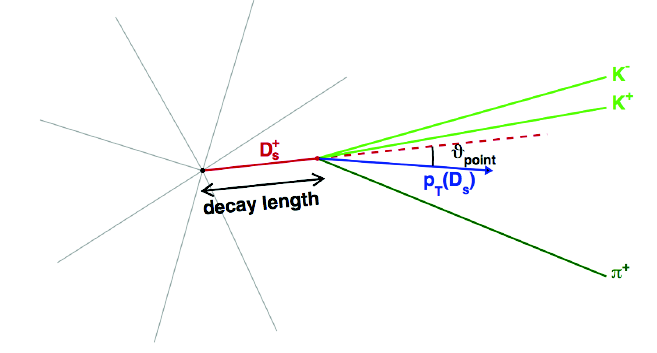
\includegraphics[width=12cm]{FigCap4/Ds.png}
\caption{Schematic view of the $\Dsplus\rightarrow \phi \pi^+ \rightarrow K^+K^-\pi^+$ decay.}
\label{fig:DsDecayTopology}
\end{figure}
Before the candidates go through specific selections of the decay
topology and particle identification, they have to pass single-track 
quality cuts. In the following, details of each selection step will
be illustrated. 



\section{Single-track selections}
Reconstructed tracks were selected by requiring:
\begin{itemize}
\item pseudo-rapidity $|\eta| < 0.8$
\item minimum $\pt > 0.3~\GeV/c$
\item at least 70 (out of a maximum of 159, i.e. number of TPC pad rows) 
associated space points in the TPC
\item $\chi^2/\mathrm{ndf} < 2$ in the TPC (where ndf is the number of degrees of 
freedom involved in the tracking procedure)
\item at least two (out of six) hits in the ITS, out of which at least one 
in either of the two SPD layers
\item ratio of crossed rows (total number of hit TPC pad rows, i.e. corrected 
for pad rows with missing signal) over findable clusters (pad rows which, 
based on the geometry of the track, are possible clusters) in the TPC larger than 0.8
\end{itemize}
For tracks that satisfy the above selection criteria, the transverse momentum 
resolution is better than 1$\%$ at $\pt = 1\, \Gevc$ and about 2\% at $\pt = 10 \, \Gevc$. 
The resolution on the track impact parameter, which is the distance of closest 
approach of the track to the primary vertex, is better than 75 $\mu$m for 
$\pt >$ 1 $\Gevc$ for the projection on the bending plane ($r\phi$, normal to 
the beam direction) in pp collisions.
In order to have unbiased determination of the primary vertex, for each 
$\Dsplus$ candidate the interaction point was recalculated from the reconstructed 
tracks after excluding the candidate decay tracks.
\begin{figure}[!htbp]
\begin{center}
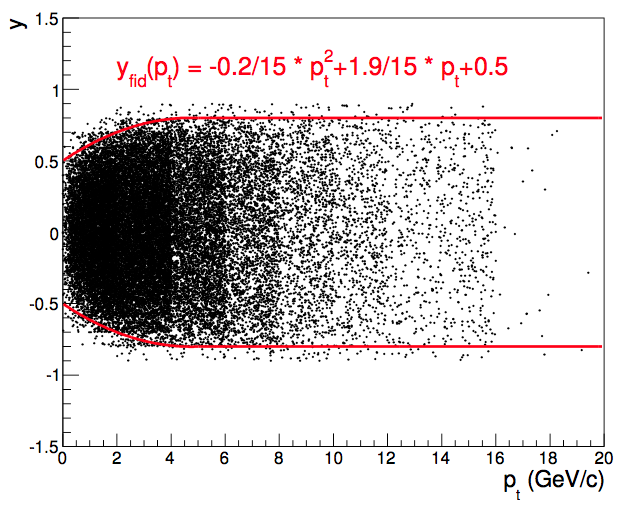
\includegraphics[width=.5\textwidth]{FigCap4/YvsPt.png}
\label{fig:singtrafter}
\caption{Rapidity versus $\pt$ distribution of the reconstructed $\Dsplus$ mesons. The fiducial acceptance region is defined by $|y| < y_{fid}(\pt)$.}
\end{center}
\end{figure}

The single-track selection criteria reduce the $\Dsplus$-meson acceptance, which drops 
steeply to zero for $|y| > 0.5$ at low $\pt$ and for $|y| > 0.8$ 
at $\pt > 5~\Gevc$. A $\pt$-dependent fiducial acceptance region was therefore defined as 
$|y| < y_{\mathrm{fid}}(\pt)$, with $y_{\mathrm{fid}}(\pt)$ increasing 
from 0.5 to 0.8 in the transverse momentum range $0 < \pt < 5~\Gevc$ 
according to a second-order polynomial function, and $y_{\mathrm{fid}}=0.8$ 
for $\pt > 5~\Gevc$.

\section{Decay-chain and topology selection}

The single-track selection provids a certain number of candidate
 decay tracks. Then, $\Dspm$ candidates are build from combinatorial 
 association of three candidate tracks, with the correct combination of charge 
 sign. In this way, a huge number of candidates is created, most of them 
 being combinatorial background. The goal is to separate background from
  $\Dspm$ signals (i.e. corresponding to real  $\Dspm$ decays). Candidates 
  are thus selected by applying topological cuts, specific to the meson and its 
  decay channel and varying as a function of the D-meson $\pt$.
The main feature of the $\Dsplus$-decay topology is the presence of three tracks displaced from 
the primary vertex and compatible with the hypothesis of being originated from 
a common point. 
The variable that allows one to evaluate the displacement of a track is the 
impact parameter. The two most important detectors for the measurement
 of the impact parameter are the two SPD inner layers of the Inner Tracking System. \\
Below, the topological cuts used for $\Dspm$ signal selection
 are explained in detail. Fig.~\ref{fig:var1},~\ref{fig:var2} and~\ref{fig:var3} complement
 the description, showing distributions of some of the below listed variables
 for signal and background candidates, in the interval $2 < \pt < 16 \, \Gevc$, 
 extracted from Monte Carlo production (PYTHIA~\cite{Sjostrand:2006za}) and data, respectively.
  New topological variables were introduced with respect to the 
  previous analysis of this sample. They are the projections of the cosine of 
the Pointing angle and of the (normalised) decay length in the $xy$ plane 
 and the single-track normalised impact parameter residual.
\begin{itemize}
\item \textbf{Decay length $D_{len}$}, defined as the distance between
 primary and secondary vertex. $\Dspm$ decay vertexes are displaced by
  a few hundred $\mu$m from the interaction vertex. Since real $\Dspm$ 
  decay vertices have, on average, larger values of decay length than the
   background, as can be seen in Fig.~\ref{fig:var1} (left), 
   this allows one to discriminate signal from background. 
   Likely cut values are $D_{len} > 300-400\, \mu $m. 
   To be noted that candidates coming from weak decays of beauty hadrons have larger $D_{len}$
   with respect to prompt $\Ds$ from charm decay, due to more displaced decay vertices.
\item \textbf{Normalized decay length $L$}, defined as the decay length 
divided by its uncertainty (Fig.~\ref{fig:var1} right).
\item \textbf{Cos$\theta_{point}$}, where $\theta_{point}$ is the angle
 between the momentum of the reconstructed $\Dspm$ meson and the 
 $\Dspm$ flight line (line connecting primary and secondary vertex, see
  left panel in Fig.~\ref{fig:var2}). The pointing angle is expected to be small for signal 
  candidates, resulting in a distribution of cos$\theta_{point}$ peaking at 1 for 
  signal and being broader for background candidates. Hence, cuts like 
  cos$\theta_{point} >$ 0.93 or tighter were usually applied to reject background.
\begin{figure}[!t]
\centering
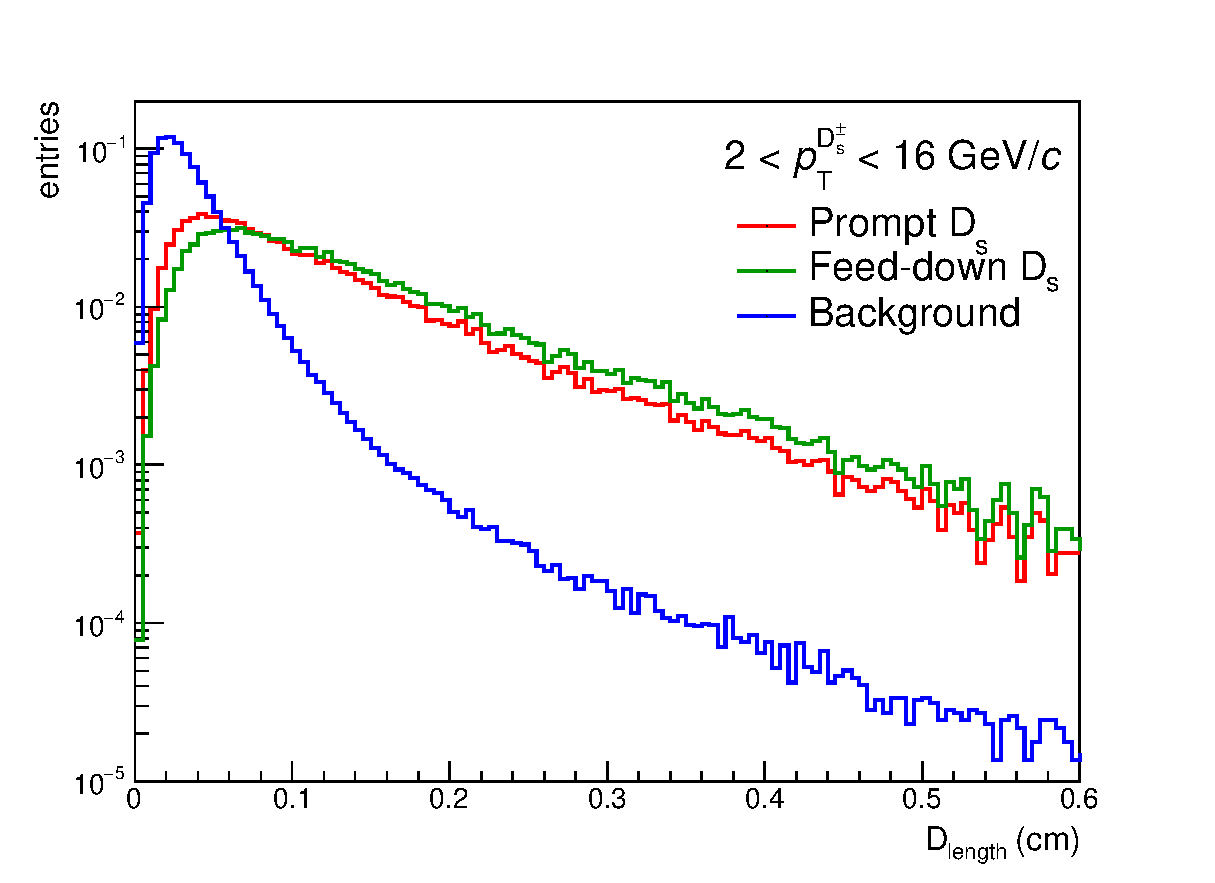
\includegraphics[width=6.5cm]{FigCap4/DL.eps}
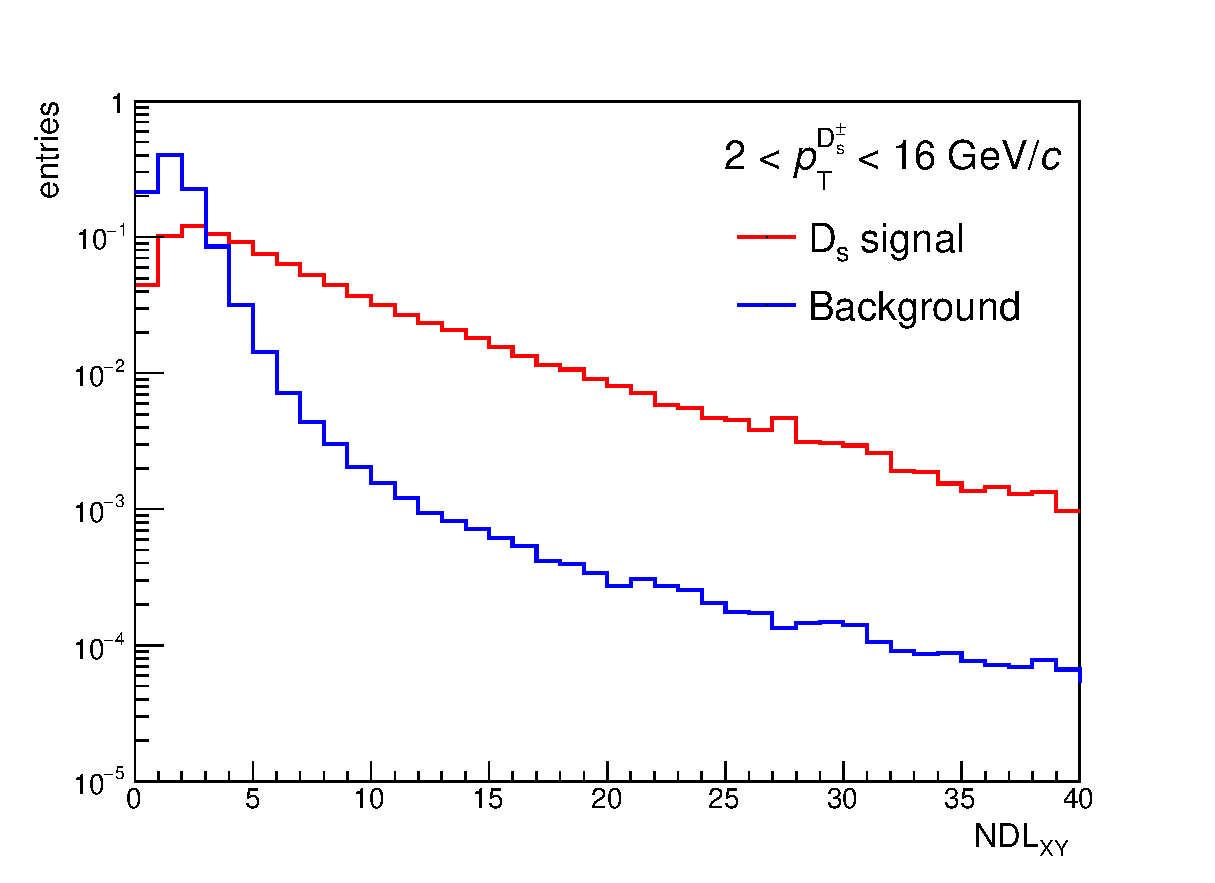
\includegraphics[width=6.5cm]{FigCap4/NDLxy.eps}
\caption{Left: distributions of decay length for prompt (red), feed-down (green) signal and background (blue) $\Ds$ candidates. Right: distributions of normalised decay length in the transverse plane signal (red) and background (blue) $\Ds$ candidates.}
\label{fig:var1}
\end{figure}
\begin{figure}[!h]
\centering
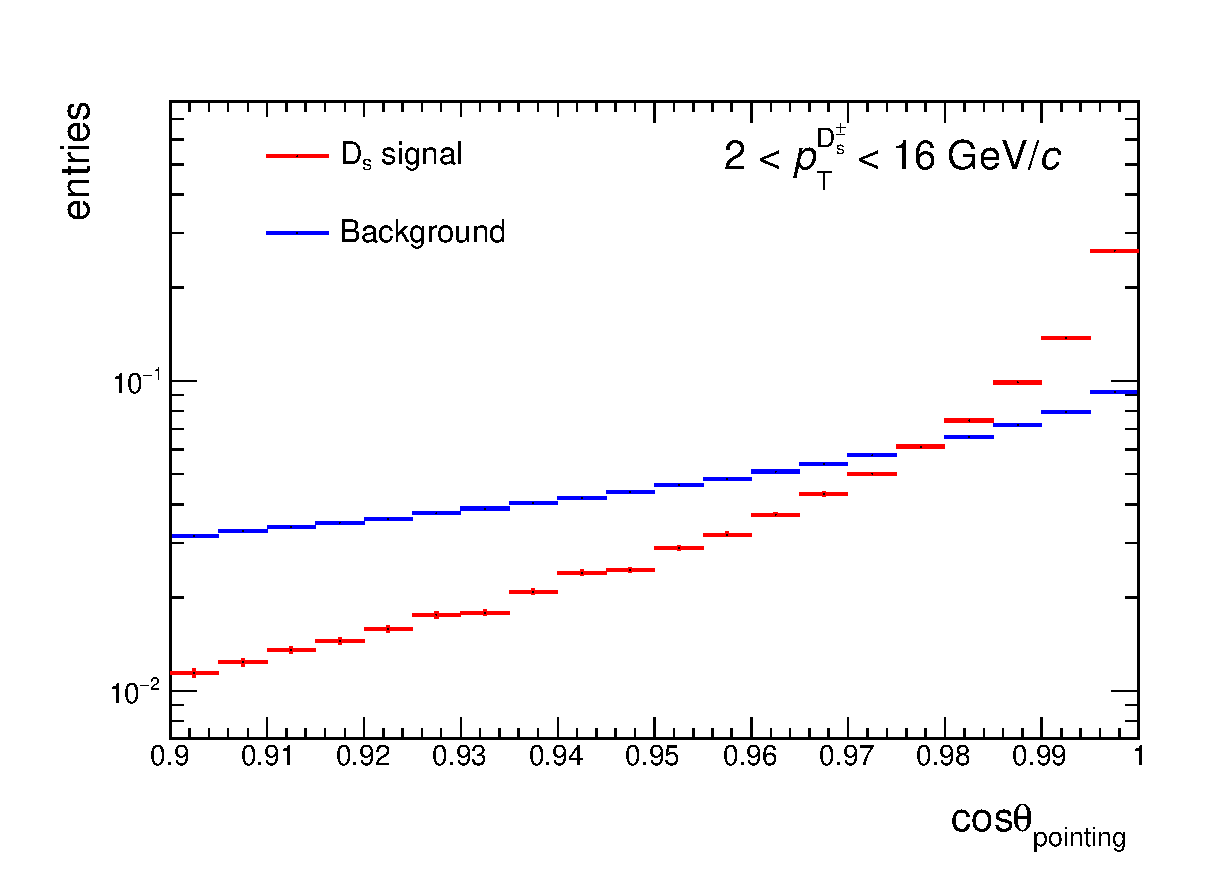
\includegraphics[width=6.5cm]{FigCap4/cosP.eps}
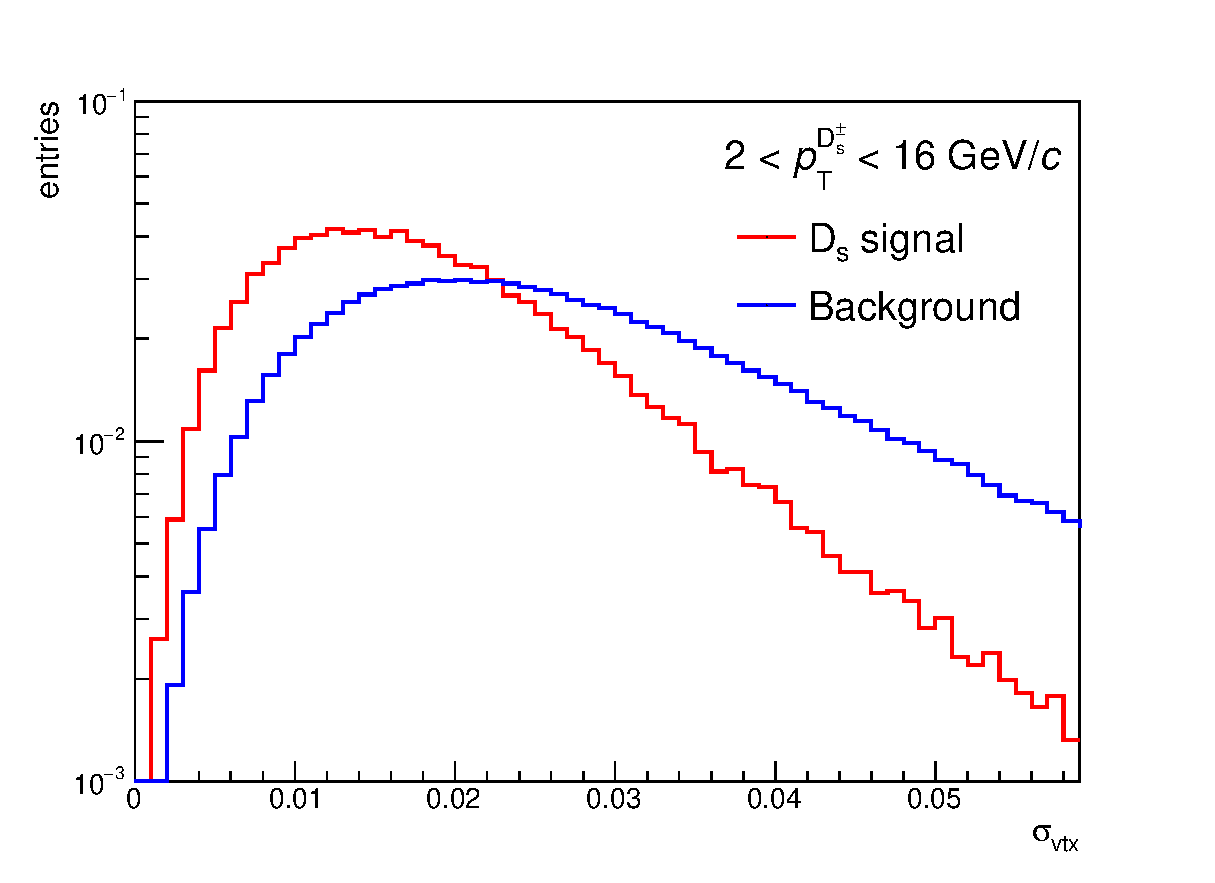
\includegraphics[width=6.5cm]{FigCap4/sigVert.eps}
\caption{Distributions of cos$\theta_{point}$ (left) and track dispersion around secondary vertex $\sigma_{vertex}$ (right) for signal (red) and background (blue) $\Ds$ candidates.}
\label{fig:var2}
\end{figure}
\begin{figure}[!h]
\centering
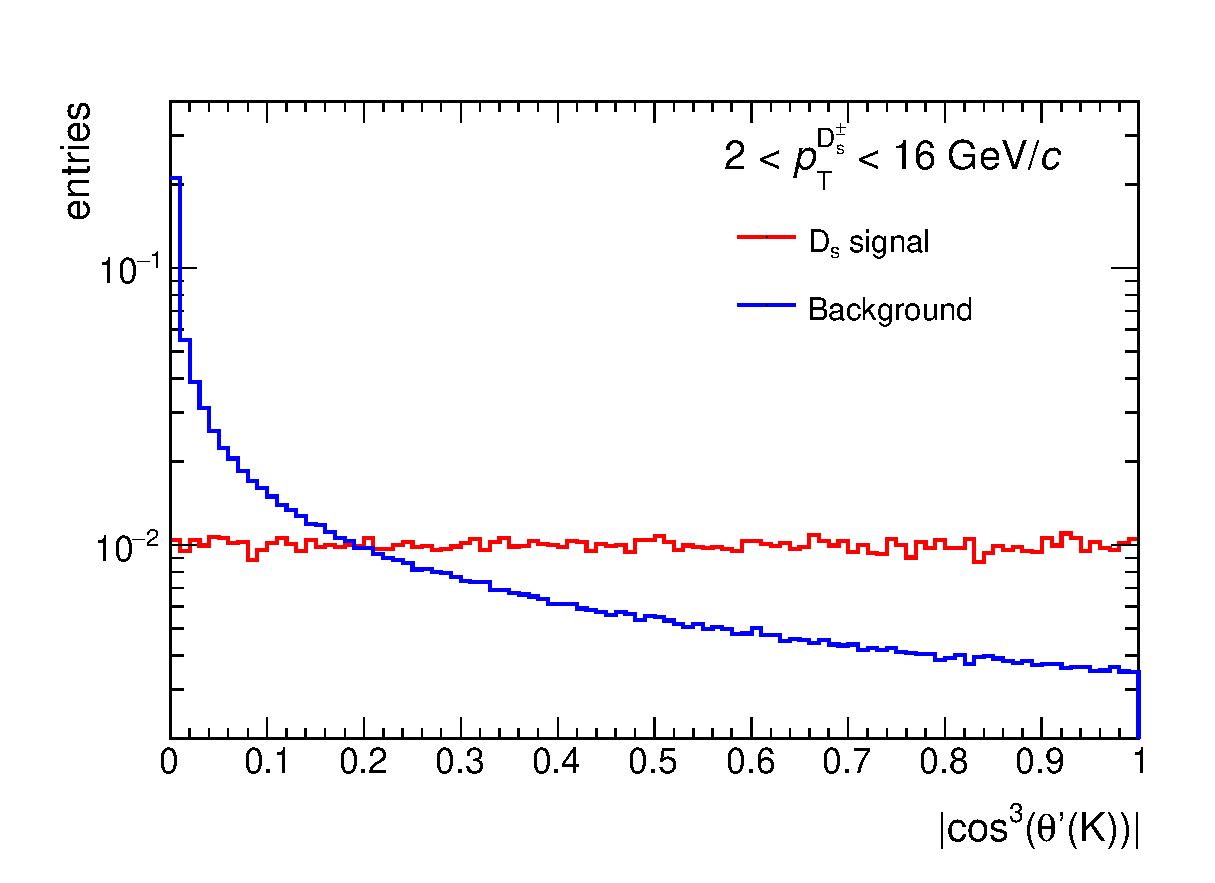
\includegraphics[width=6.5cm]{FigCap4/CosPiKPhi3.eps}
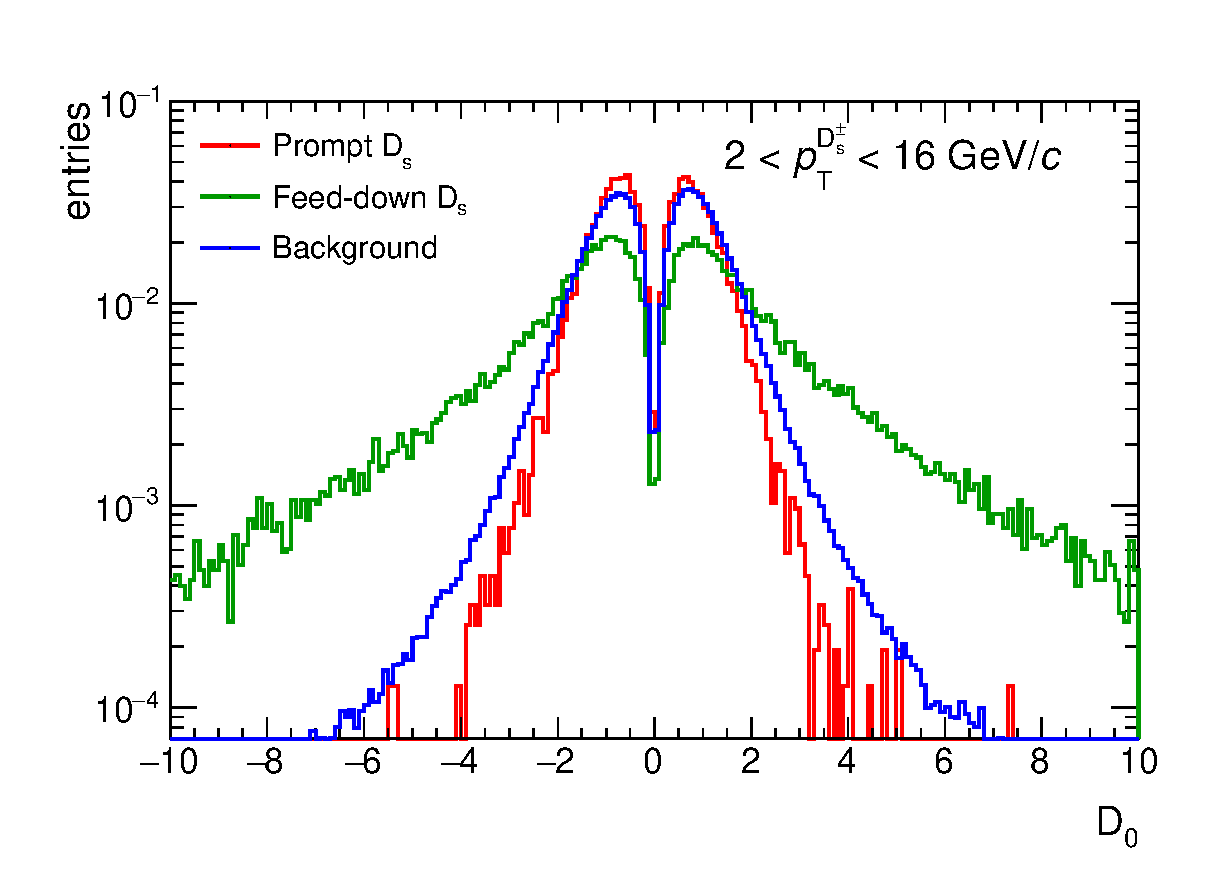
\includegraphics[width=6.5cm]{FigCap4/normIP.eps}
\caption{Left: distributions of $|cos^3(\theta'(K))|$ for signal (red) and background (blue) $\Ds$ candidates. Right: distributions of normalised decay length in the transverse plane for prompt (red), feed-down (green) signal and background (blue) $\Ds$ candidates.}
\label{fig:var3}
\end{figure}

\item \textbf{Track dispersion $\sigma_{vertex}$} around the decay vertex, defined as:
\[
\sigma_{vertex}=\sqrt{d^2_1+d^2_2+d^2_3}
\]
where $d_i$ is the distance of minimal approach between the decay 
track \textit{i} and the decay vertex. All tracks should originate from 
the secondary vertex, and $\sigma_{vertex}$ should be $\sim$ 0; in 
real cases, as a consequence of the tracking and vertexing resolution, 
the $\sigma_{vertex}$ has non-zero values and an upper cut is needed 
to exclude vertices made of random combination of tracks. Typical cut
 values on the track dispersion were between 0.02 $< \sigma_{vertex}<$ 0.05 cm 
 (see Fig.~\ref{fig:var2} right).
\item \textbf{$\theta^*(\pi)$ angle}, it is the angle between the pion 
in the KK$\pi$ rest frame and the KK$\pi$ flight line. Cuts were applied
 on the distribution of the cos$\theta^*(\pi)$, with typical values 
 between 0.95 $<cos\theta^*(\pi)  <$ 1.0.
\item \textbf{$\theta'$(K) angle}, it is defined as the angle between
 one of the kaons and the pion in the KK rest frame. Cuts were 
 applied on the distribution of the $|cos^3(\theta'(K))|$ (Fig.~\ref{fig:var3}, left), with typical 
 values between 0.0 $<|cos^3(\theta'(K))| <$ 0.05.
\item \textbf{Single-track normalised impact parameter residual $IP$} : it is defined 
as the difference between the expected 
impact parameter value $d^{exp}_{0,r,\phi} \approx D_{len}^{xy} \cdot sin(\theta_{xy})$
 ($D_{len}^{xy}$ is the decay length on $xy$ plane and $\theta_{xy}$ is the angle 
between the reconstructed D meson and the $i$-th daughter track on $xy$ plane) 
and the reconstructed one $d^{reco}_{0,r,\phi}$ for the $i$-th daughter
track, then normalised by the square 
root of their respective uncertainties summed in quadrature. 
In Fig.~\ref{fig:var3} (right) the distributions of the maximum $IP$ among 
the three daughter tracks of $\Ds$ candidates are shown, in different colours for
background and true candidates, distinguished between prompt and beauty 
feed-down components. Since the distributions of the normalised $IP$ residuals 
are quite different for prompt and feed-down D mesons, 
a selection based on this variable can reduce the feed-down D-meson efficiency while keeping 
higher that of prompt D mesons. In this analysis selections on the single-track $IP \sim 2$
were applied.
\end{itemize}

The selections on $\theta^*(\pi)$ and $\theta'$(K) angles have already 
been used in various experiments which measured $\Dsplus$ production 
like ZEUS \cite{Chekanov:2005mm} and ATLAS \cite{ATLAS:2011fea} as well as 
in previous ALICE analyses~\cite{ALICE:2011aa,Abelev:2012tca,Adam:2016ich,Adam:2015jda}
 and are based on kinematical 
considerations on the decay chain with a $\phi$ in the intermediate state.
Further selections were applied on the projections of the decay length, 
the normalized decay length and the cos$\theta_{point}$ in the transverse 
plane $xy$. The projections of the variables in the $xy$ plane are instead justified by 
the improving of the impact parameter resolution with respect to $z$-direction.\\


A further parameter which allowed to reduce the background is the
 \textbf{invariant mass of the reconstructed $K^+K^-$ pair}. This is not a topological 
 cut (i.e. a cut exploiting the displacement of the decay vertex), 
 but rather a selection on the decay chain. It is required that at least 
 one of the two pairs of tracks with opposite charge has an invariant
  mass compatible with the $\phi$ mass. The selection is done on 
  the absolute value of the difference between the $\phi$ 
   invariant mass from PDG and the reconstructed one:
\[
\Delta M = |M^{inv}_{rec}-M_{\phi}|.
\]
Typical values for cuts on $\Delta M$ are between 3 $<\Delta M<$ 15 MeV$/c^2$.

\section{Particle identification}
\label{Sec:PID}
The Particle IDentification (PID) selection is based on the specific energy loss 
d$E$/d$x$ in the TPC and the time-of-flight from the interaction vertex to the 
TOF detector. This is used in the D-meson analysis to reduce the background, 
but it is essential for $\Dsplus$ studies because low values of signal-over-background
 ratios (S/B).
A track is  considered compatible with a certain particle species 
($\pi$, K or p) if the measured signal has a difference 
within $n\sigma$ from the expected one for the various mass hypotheses
  with the theoretical predictions:
\[
|S_{meas}-S^{\pi,k,p}_{expected}| < n^{\pi,k,p}\sigma ,
\]
where $\sigma$ is the RMS of the Gaussian fit of the theoretical 
curve to the energy-loss or time-of-flight signals for each species.
Candidate triplets were required to have two tracks compatible with 
the kaon hypothesis and one with the pion hypothesis. In addition, 
since the decay particle with opposite charge sign has to be a kaon, 
a triplet was rejected if the opposite-sign track was not compatible 
with the kaon hypothesis. 
The criterion used to classify tracks on the basis of their PID
information in TPC and TOF detectors is 
illustrated in Fig.~\ref{fig:strongPID}, where $n\sigma^{\rm max,TPC} = 1$ for
$0.6 < \pt < 0.8 \, \Gevc$ and 2 elsewhere and $n\sigma^{\rm max,TOF} = 3$ at all $\pt$.  
To combine PID information in the two detectors,
the response values in TPC and TOF (green values in Fig.~\ref{fig:strongPID}) 
are summed linearly together 
and the track is considered
compatible with a species hypothesis if the combined response value is 1 or 2. This
PID selection preserves $\sim$85-90\% of the signal depending on the $\pt$.

 
\begin{figure}[!h]
\centering
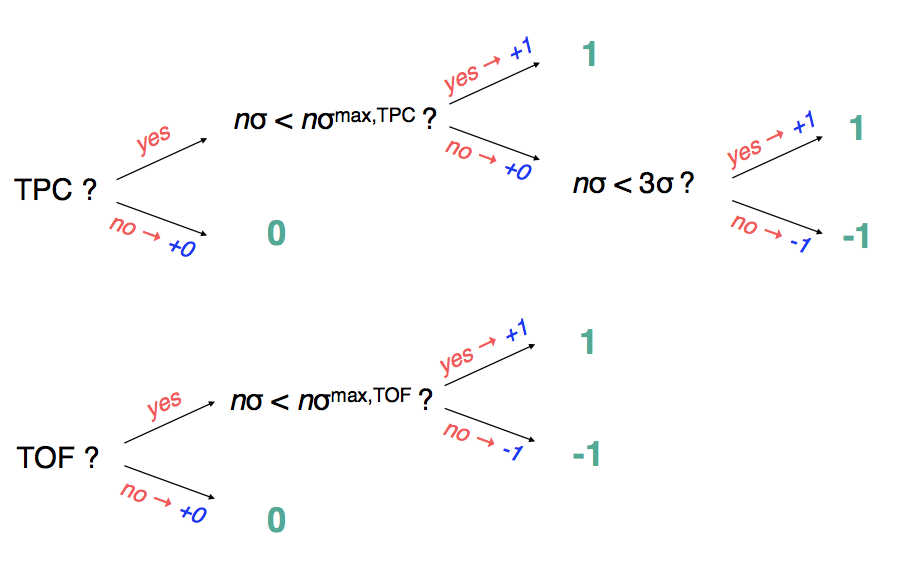
\includegraphics[width=11cm]{FigCap4/strongPID.png}
\caption{PID selection criteria in TPC and TOF for a specific mass hypothesis.}
\label{fig:strongPID}
\end{figure}


\section{Invariant mass spectra and signal extraction}
For each candidate, two values of invariant mass can be computed, 
corresponding to the two possible assignments of the kaon and the 
pion mass to the two same-sign track. In fact, considering the $\Dsplus$
 decay, the charge configuration of the tracks (+, -, +) can be interpreted
  both as to ($K^+,K^-,\pi^+$) and ($\pi^+,K^-,K^+$). Signal candidates with 
  wrong mass assignement to the same-sign tracks would give rise to 
  a contribution to the invariant mass distributions that could introduce
   a bias in the raw yield of $\Dsplus$ mesons. It was verified, both in 
   data and in simulations, that this contribution is reduced to a negligible 
   level by particle identification selection and by the requirement that the
    invariant mass of the two tracks identified as kaons is compatible with 
    the $\phi$ PDG mass.

Once that $\Dsplus$ candidates pass the selections they are 
used to fill invariant mass histograms in different $\pt$ intervals.
The histograms are fitted by a function consisting of a sum of 
a Gaussian and an exponential function to describe the signal peak and 
the background shape respectively:
\begin{equation}
f(x)= Ae^{-B\cdot x}+Ce^{-\frac{(x-\mu)^2}{2\sigma^2}}.
\end{equation}
The selected criterion for the yield extraction is a particle selection 
 strategy that preserves high selection efficiency and high statistical 
 significance for the D meson signal, defined as:
\[
Signif = \frac{S}{\sqrt{S+B}},
\]
where S and B are the extracted signal and background obtained 
from the fit procedure integrated within 3$\sigma$ 
around the peak of the Gaussian shape ($\sigma$ being the
RMS of the peak from the fit). The statistical significance is related to the 
relative statistical uncertainty on the extracted signal, so higher 
significance means lower statistical uncertainty on the raw yield. 
A second variable which is used in the cut optimisation procedure
 is the signal-over-background ratio S/B, as 
 an estimator of the powerfulness of the selection strategy. 
 The maximisation of the significance was required together
  with the request that the position of the peak and the width 
  of the Gaussian shape were compatible with the values
   obtained in simulated events, with the same selection strategy.
Since the topological variables have a certain degree of correlation among them, 
for each $\pt$ interval, different variables 
were simultaneously varied in wide ranges to consider all possible combinations. 
The selection values depend on the $\pt$ of the $\Ds$-meson candidate and 
are detailed in Table~\ref{tab:cutsDs}.
\begin{table}[tbh!]
\centering
\begin{tabular}{|l|c|c|c|c|} 
\hline 
 $\Ds$ meson& \multicolumn{4}{c|}{pt interval (GeV/$c$)}\\
\hline
 & 2--4  & 4--6 & 6--8 & 8--12\\
\hline
Decay length ($\mum$)        & $>$300 & $>$350 & $>$350 & $>$400\\
Decay length XY ($\mum$)     & $>$0 & $>$200 & $>$200 & $>$200\\
Norm Decay length XY          & $>$2.0& $>$0.0 & $>$2.0 & $>$2.0\\
Cosine pointing              & $>$0.94 & $>$0.95 & $>$0.95 & $>$0.97\\
$\sigma_{vertex}$  (cm)          & $<$0.02 & $<$0.03 & $<$0.03 & $<$0.06\\
$\Delta M$ (MeV/$c^{2}$) & $<$8.0 & $<$10.0 & $<$4.5 & $<$9.0\\
$\cos \theta^*(\pi)$    & $<$1.0 & $<$1.0 & $<$1.0 & $<$0.95\\
$|\cos^3 \theta^\prime({\rm K})|$        & $>$0.10 & $>$0.05 & $>$0.05 & $>$0.05\\
Norm. IP residual Kaon  & $<$2.5 & $<$2.0 & $<$2.0 & $<$2.0 \\
Norm. IP residual Pion  & $<$2.5 & $<$2.0 & $<$2.0 & $<$2.0 \\[1ex]
\hline
\end{tabular}
\caption{Selections used for the $\Dspm$ meson in the four transverse momentum intervals considered.} 
\label{tab:cutsDs}
\end{table}
In Fig.~\ref{fig:invmassDs} the invariant mass distributions 
of $\Dspm$ mesons in four $\pt$ intervals from 2 to 12 $\Gevc$ are shown 
and in Tabletab:signalDs the values of S/B, statistical significance and extracted yields are reported.
\begin{figure}[!htb]
\begin{center}
 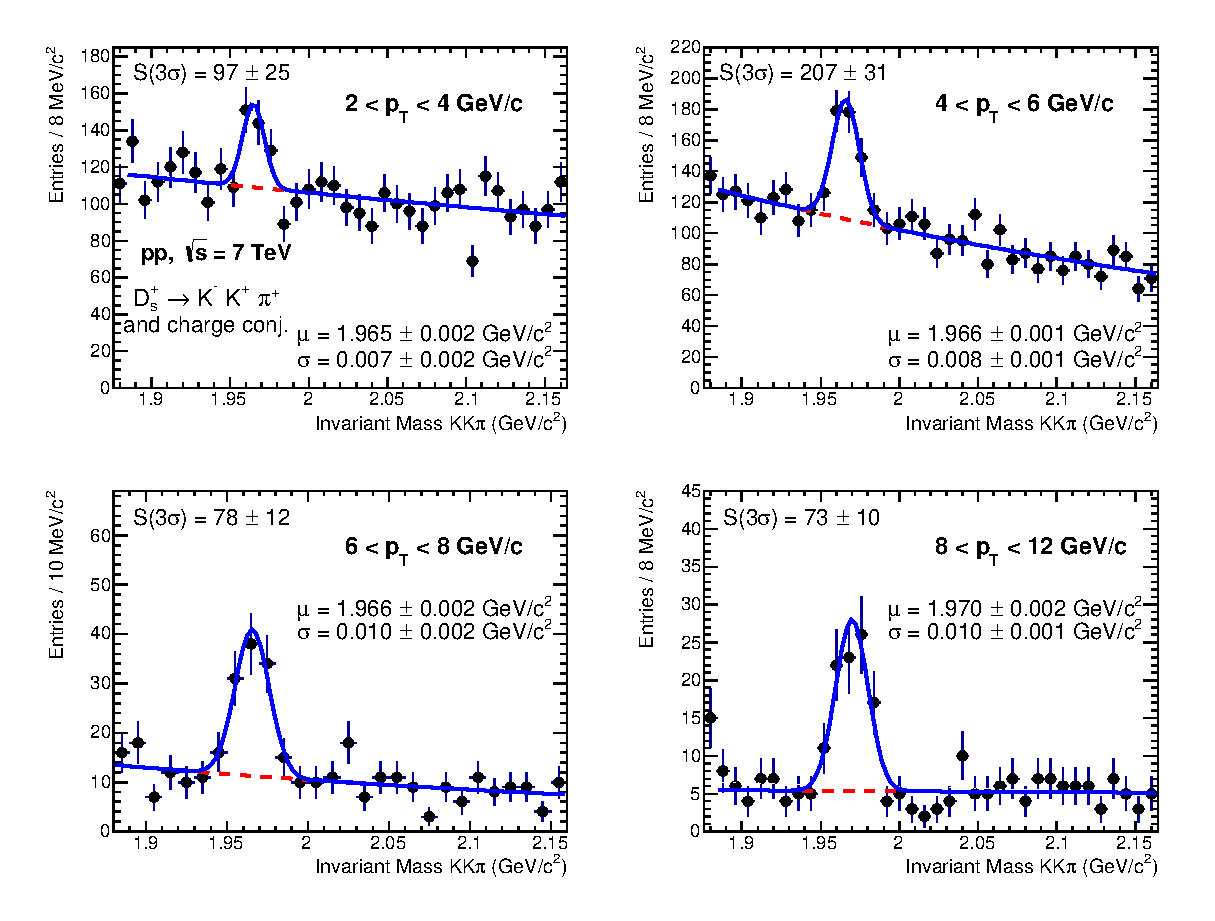
\includegraphics[width=.99\textwidth]{FigCap4/DsMassHistos_ppPass4.eps}
\caption{Invariant mass distributions of $\Dspm$ candidates and charge
conjugates in the four considered $\pt$ intervals.}             
\label{fig:invmassDs}
\end{center}
\end{figure}
\begin{table}[tbh!]
\centering
\begin{tabular}{|l|c|c|c|} 
\hline
 $\pt$ ($\Gevc$) & S/B  & Signif. & S(3$\sigma$)\\
\hline
2-4   & 0.18 & 3.8 & 97 $\pm$  25\\
4-6    & 0.30 & 6.9 & 207 $\pm$ 31\\
6-8    & 1.10 & 6.4 & 78 $\pm$ 12\\
8-12  & 1.78 & 6.8 & 73 $\pm$ 10\\
\hline
\end{tabular}
\caption{S/B, statistical significance and yield for $\Dspm$ signal peak in the four transverse momentum intervals considered.} 
\label{tab:signalDs}
\end{table}

An indication of the improved resolution provided by the new 
reconstruction of the sample is shown in Fig.~\ref{fig:sigma4vs2}, where the 
Gaussian sigmas of the invariant mass fits are shown in comparison to 
results of the previous reconstruction, for both data and MC. 
\begin{figure}[!hb]
\begin{center}
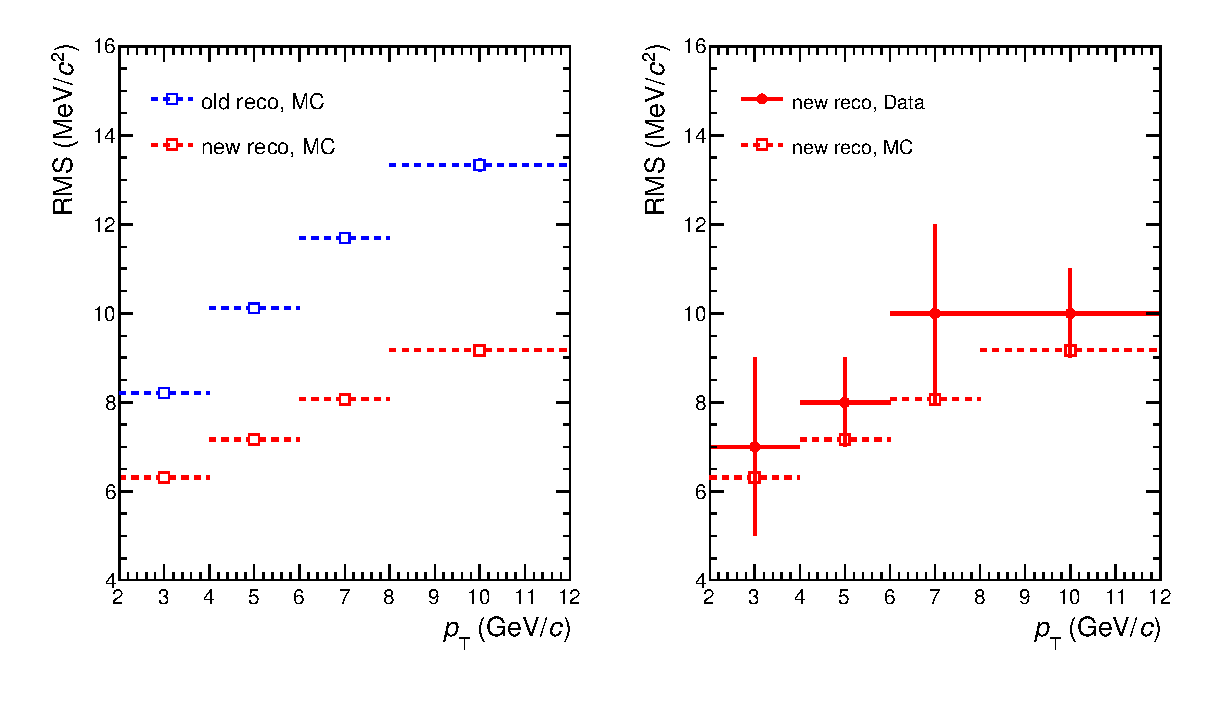
\includegraphics[width=.48\textwidth]{FigCap4/Resolutions_pass2_pass4.eps}
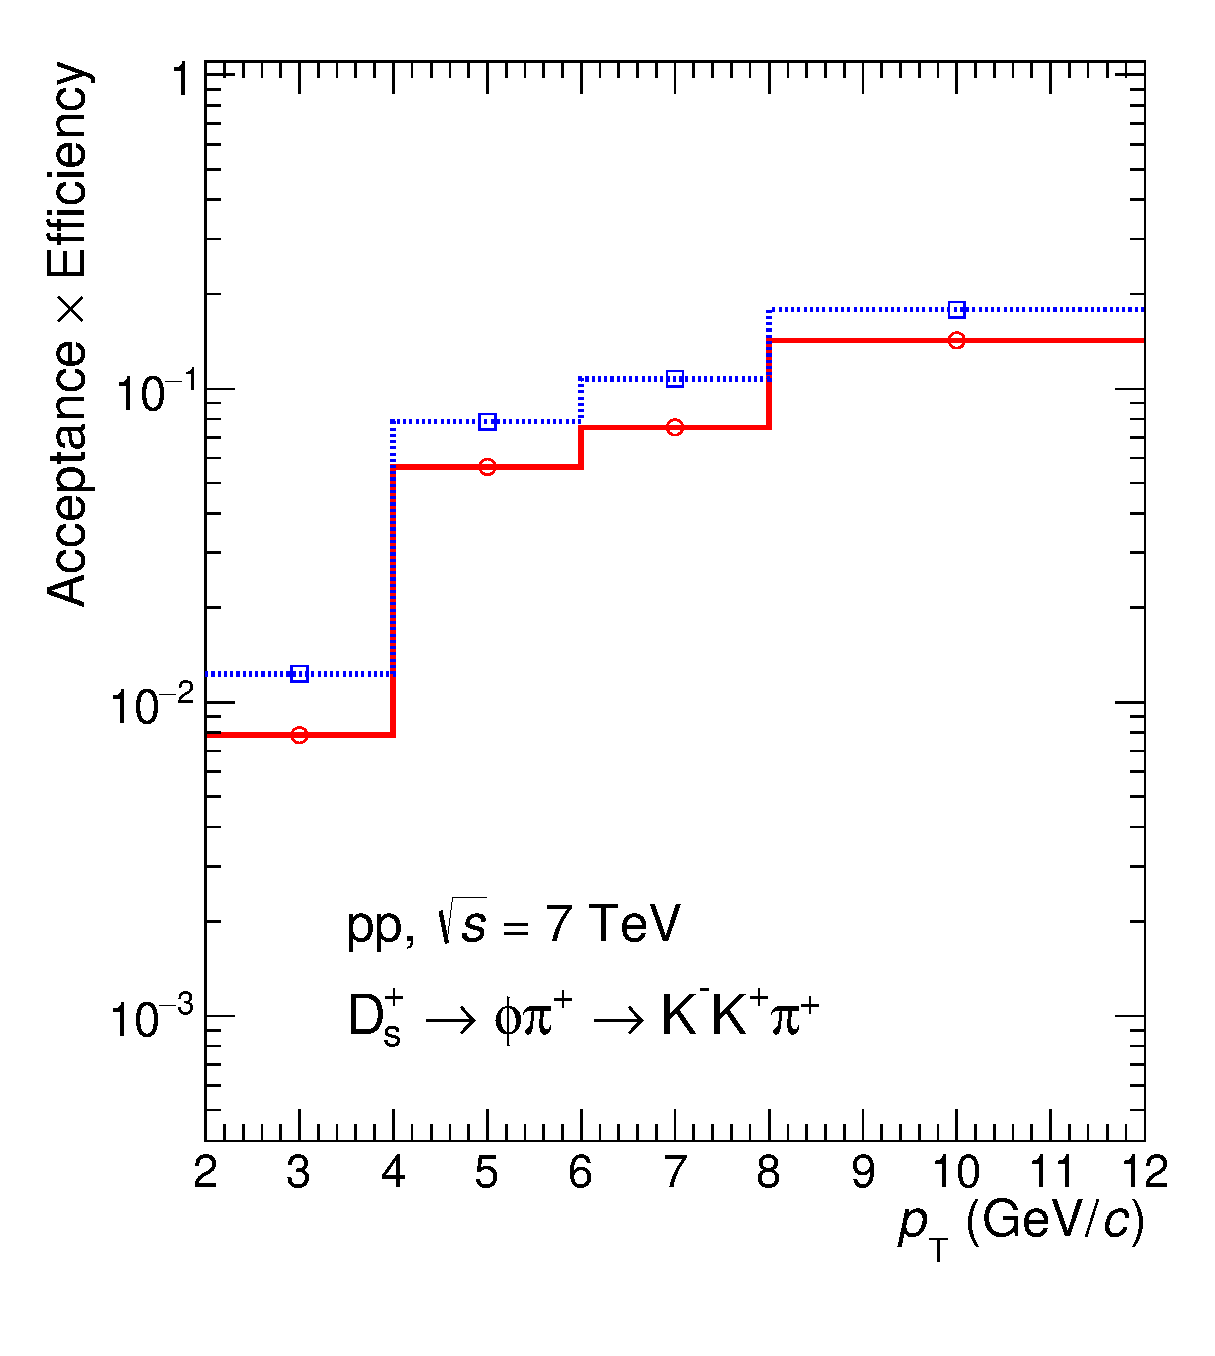
\includegraphics[width=.48\textwidth]{FigCap4/AccEff_Ds_Pass4.eps}
\caption{Left: Gaussian widths of $\Ds$ peak as a function of $\pt$, for current (red) and previous (blue) reconstruction, in data (solid) and MC (dashed). Right: acceptance-times-efficiency of prompt and feed-down $\Ds$ mesons.}
\label{fig:sigma4vs2}
\end{center}
\end{figure}

\section{Corrections}

The $\Dspm$ raw yields extracted from the fits to the invariant-mass distributions
were corrected to obtain the $\pt$-differential production cross sections of prompt
 D mesons. The production cross section was calculated as:
\begin{equation}
  \label{eq:dsdpt}
  \left.\frac{{\rm d} \sigma^{\rm D^{+}_{\rm s}}}{{\rm d}\pt}\right|_{|y|<0.5}=
  \frac{1}{ \Delta \pt}\frac{1}{{\rm BR} \cdot L_{\rm int}}\frac{\left.f_{\rm prompt}(\pt)\cdot \frac{1}{2} N^{\rm D^\pm_{\rm s}~raw}(\pt)\right|_{|y|<y_{\rm fid}}}{ 2 y_{\rm fid}(\pt) \,({\rm Acc}\times\epsilon)_{\rm prompt}(\pt)}\,,
\end{equation}
where $N^{\rm D^\pm_{\rm s}~raw}(\pt)$ is the value of the raw yield 
(sum of particles and antiparticles),
 which needs to be corrected for the B-meson decay feed-down contribution 
(i.e.\ multiplied by the prompt fraction $f_{\rm{prompt}}$), divided by the 
acceptance-times-efficiency term for prompt $\Ds$ mesons 
$(\rm Acc \times \epsilon)_{\rm{prompt}}$, and divided by a factor of two to 
obtain the charge (particle and antiparticle) averaged yields.
The corrected yields were further divided by the decay channel branching ratio (BR), 
the $\pt$ interval width ($\Delta \pt$), the rapidity coverage 
($2 y_{\rm fid}$) and the integrated luminosity $L_{\rm int}$.
The rapidity acceptance correction factor $\Delta y=2\,y_{\rm fid}$ assumes
a uniform rapidity  distribution for D mesons in the measured $y$ range.
This assumption was verified to the $1\%$ level with PYTHIA proton-proton simulations 
with the Perugia-0 tuning.
The integrated luminosity was computed as $L_{\rm int} = N_{ev}/\sigma_{pp,MB}$,
where $N_{ev}$ is the number of analysed events and 
$\sigma_{pp,MB} = 62.2$ mb~\cite{Abelev:2012sea}
is the cross-section for the minimum-bias trigger condition, derived from
a van der Meer scan measurement~\cite{vanderMeer:296752}.

\subsection{Reconstruction and selection efficiency}
The acceptance-times-efficiency correction factor, 
$(\rm Acc \times \epsilon)$, was determined for the $\Ds$-meson
hadronic decay considered in this analysis using Monte Carlo simulations 
of pp collisions generated with the PYTHIA 6.4.21 event generator~\cite{Sjostrand:2006za} with the 
Perugia-0 tune~\cite{Skands:2010ak} and particle transport through the apparatus 
using GEANT3~\cite{Brun:1994aa}.
The luminous region distribution and the conditions (active channels, gain, 
noise level and alignment) of all the ALICE detectors were included in the 
simulations, considering also their evolution over time during the 2010 LHC 
data taking period.
In the production, only events containing a $c\bar{c}$ or a $b\bar{b}$ pair 
were transported through the apparatus and reconstructed and
D mesons were forced to decay hadronically via the decay channel relevant to
the specific analysis.
The efficiency was extracted separately for prompt and feed-down D-mesons and 
is shown in the right panel of Fig.~\ref{fig:sigma4vs2}.
D mesons from beauty decay have higher efficiency than
the prompt ones in all the $\pt$ intervals, due to the more displaced 
decay vertex from interaction point.
In general, with the chosen topological selections, efficiencies in this analysis
are on average 15\% lower than those used in the previous reconstruction. 
The present analysis uses more powerful selection variables 
(projections on $xy$ plane and impact parameter residual) that
enhance the signal-over-background ratio for $\Ds$ meson by a factor 
from 2 to 5 depending on the $\pt$ interval, with an acceptable worsening
of the global efficiency. Large signal-over-background ratios are indeed essential 
to assure a good stability of the extracted yield.

\subsection{Beauty feed-down subtraction}

The $f_{\rm prompt}$ fraction was calculated using the beauty production cross sections from  
FONLL calculations~\cite{Cacciari:1998it, Cacciari:2001td}, the 
$\mathrm{B} \rightarrow \mathrm{D} + X$ decay kinematics from the EvtGen package~\cite{Lange:2001uf} 
and the efficiencies for feed-down D mesons reported in 
Fig.~\ref{fig:sigma4vs2} (right):
\begin{equation}
\label{eq:fpr}
\begin{split}
f_{\mathrm{prompt}} = \, & 1- \frac{N^{\text{D~feed-down}}_{\mathrm{raw}}}{N^{\mathrm{D}}_{\mathrm{raw}}}=\\
& 1- \left (\frac{\rm d^2 \sigma}{\mathrm d\pt \mathrm d y} \right)^{\rm FONLL}_{\text{feed-down}} \cdot \frac{(\mathrm{Acc} \times \epsilon)_\text{feed-down} \cdot \Delta y \Delta \pt \cdot \mathrm{BR} \cdot L_{\rm int}}{N^{\rm D +\overline{D},raw}/2}\,,
\end{split}
\end{equation}
where the $\pt$ dependence of $f_{\rm prompt}$, $N^{\rm D +\overline{D},raw}$ and
$(\mathrm{Acc} \times \epsilon)_\text{feed-down}$ is omitted for brevity.
The values of $f_{\rm prompt}$ of $\Ds$ meson are shown in Fig.~\ref{fig:fprompt} as a function of $\pt$.
\begin{figure}[!t]
\begin{center}
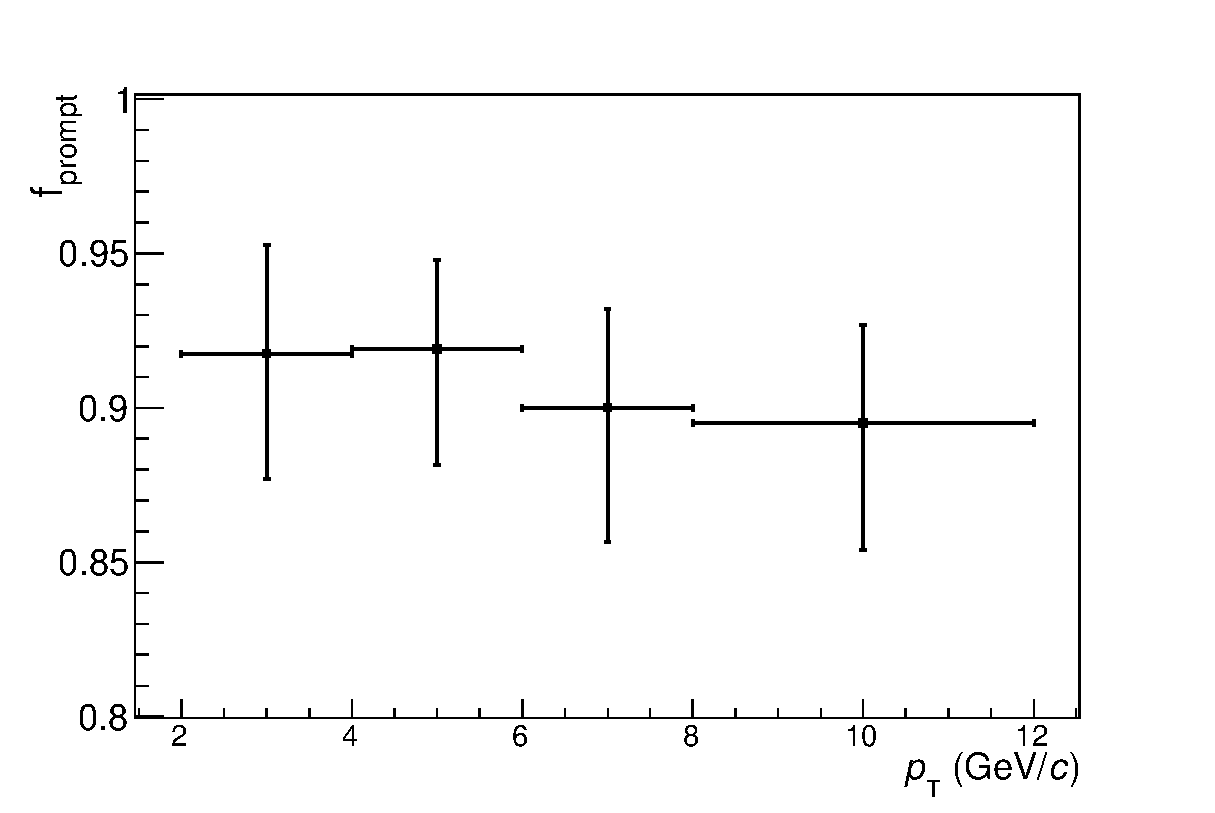
\includegraphics[width=.48\textwidth]{FigCap4/promptFraction_pass4.eps}
\caption{Prompt fraction values for $\Ds$ meson with the final selections as a function of $\pt$ in pp collisions at $\s = 7$ TeV.}
\label{fig:fprompt}
\end{center}
\end{figure}



\section{Systematic uncertainties}
\label{sec:systPP}
In this section the study of the systematic uncertainties for the
 measurement of the $\Dsplus$ cross section as a function of $\pt$ is presented. 
 The contributions to the systematic uncertainty from different 
 sources were studied separately and described in detail in the following.

\subsection{Raw yield extraction}
\label{sec:RawYieldSyst}
Fluctuations of the extracted yields are observed when varying fit 
configurations. 
In order to keep under control variations of the raw yields, a possible
approach is to explore all the possible fit configurations and build
a distribution of the yields. The fits to the invariant-mass 
distributions were repeated several times varying
i) the invariant-mass bin width, ii) lower and upper limit of the fit, 
iii) background fit function (3 cases: exponential, linear and second 
order polynomial), iv) Gaussian mean and width of the signal line shape 
free of fixed to MC
values. The fits which did not converge or had $\chi^2$/ndf $>$ 2.0 
were rejected and not considered in the evaluation of the 
systematic uncertainty. It was verified that the yields extracted with the
default fit parameters had similar values to the mean of
the distribution of yields from multiple trial fits. 
The RMS of such distributions can be used as an estimator of
the systematic uncertainty on the extraction and, with the above
selection criteria, their values result $\sim$6\%.
In addition, the results obtained with 
the fitting technique were compared to those obtained by 
counting the entries in the invariant mass histogram after 
subtracting the background counts calculated from the 
background fit function and their relative difference resulted
to be smaller than 6\%. 
To further investigate whether the estimate of the systematic uncertainty
derived from this approach is not to much conservative, a slightly
different approach was tested. We assume that 
possible systematics on the yield extraction via fit procedure 
arise only from variations in the line shape of the signal and 
in the fitting function for the 
background. Let's examine these two contributions separately.\\

\emph{Signal line shape}
The uncertainty from signal line shape was calculated by 
considering the combinations among these fit
configurations: (i) free Gaussian width parameter, (ii) width parameter 
fixed to MC value, (iii) width parameter varied by 20\% with 
respect to MC value,  (iv) free mean parameter, (v) mean parameter fixed to MC value.
The error was extracted as the maximum error (max. value - min. value) divided by $\sqrt{12}$.
It resulted in a $\sim$5\% systematic uncertainty in all the $\pt$ intervals.

\begin{table}[!t]
\centering
\vspace{0.5cm}
\begin{tabular}{|c|c|c|c|c|} 
\hline \rule{0pt}{2.7ex}
 & $\pt$ interval & Exponential & Linear & Pol2 \\ 
 &(GeV/$c$) & & &  \\ 
\hline \rule{0pt}{2.7ex}
           &\phantom{0}2--4\phantom{0} & 1.21 & 1.21 & 1.09\\
           $\chi^2/ndf$ &\phantom{0}4--6\phantom{0} & 1.15 & 1.18 & 1.16\\
          &\phantom{0}6--8\phantom{0} & 1.03 & 1.02 & 1.03\\
           &\phantom{0}8--12 & 0.99 & 0.99  & 1.03\\
\hline
\end{tabular}
\caption{Reduced $\chi^2$ values for the fit of the background (peak region excluded) in the
considered $\pt$ intervals of the $\Ds$ meson.} 
\label{tab:chi2bkg}
\end{table}

\begin{figure}[!hb]
\begin{center}
 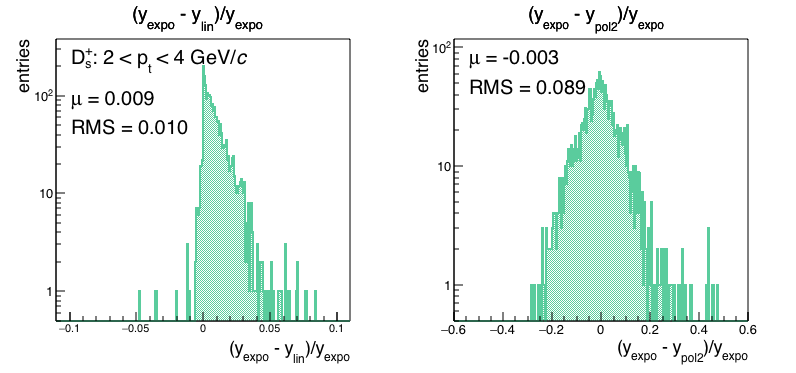
\includegraphics[width=.70\textwidth]{FigCap4/studyBkg_Free_pt0.png}
\caption{Relative difference of signal yield with exponential and first (left) and second (right) 
order polynomial functions for background, in $2 < \pt < 4 ~\Gevc$.}             
\label{fig:diffBkgPt0}
\end{center}
\end{figure}


\emph{Background fit function}
Using different functions to fit the background could in 
principle introduce some systematic difference in the extracted yields.
The default shape used to give the central yield is an 
exponential function, but first and second 
order polynomial shapes were also tested. In Table~\ref{tab:chi2bkg} 
the values of reduced chi square referred to the compatibility 
of the background function with data (excluding peak region) are 
reported. One can see that all the three shapes 
give a good description of data, but in general no improvements 
are visible when adding more parameters in the fit
with respect to exponential shape, so the latter confirms itself as a good choice.
Neverthless, it is important to look also at the values of the 
extracted yield to assess about possible biases.
 In order to do this, 50 simulated samples were generated via 
 Poissonian smearing of the fit function with the exponential background.
 For each sample, yields extracted with exponential 
 background were compared with those using linear and 
 polynomial functions with the same
configuration for pole, sigma, mass range and bin width, and their
difference, normalised to the yield extracted using a fit with exponential background, 
was used to fill a histogram. The procedure was repeated for different
configurations of lower and upper limits for the fit and 
invariant-mass bin widths for each of the
50 samples. 
A potential shift from zero of the mean of the resultant distribution 
 should reveal the bias from the change of background. The
  spread of the distribution is related to statistical fluctuations. 
  In Fig.~\ref{fig:diffBkgPt0} an example of the above 
  described distribution is presented, in the interval $2 < \pt < 4\, \Gevc$.
  Left and right panels show respectively the distribution of the difference
  of yields extracted with first or second order polynomial shapes to those extracted with exponential
  background. The shift in the distribution is not statistically significant 
 since $\mu < 3\,$RMS.\\
 
 
 
 
The systematic of yield extraction from the second approach is hence $\sim$5\%, which
is consistent with the $\sim 6$\% found with the first approach. 
It results reduced by a factor 3-4 with respect to the analysis of the old reconstrunction,
where it was around 15-20\% depending on the $\pt$ interval. 

\subsection{Selection efficiency}
\label{sec:CutVariation}
The systematics on the selection efficiency accounts for 
possible imperfections in the MC description ($\pt$, 
impact parameter resolution) which could 
impact the raw yield correction via the efficiency term.
A possible test to quantify the effect of imperfections in the 
description of topological variables in the MC is to exploit different sets of cuts
that have different selection efficiencies and to compare the corrected
yields. In this analysis, twelve sets of cuts with 
medium-high statistical significance of the extracted yields were compared, 
their respective efficiencies spanning a variation of
a factor from 2 to 6, depending on the $\pt$ interval, between minimum 
and maximum efficiency considered. We take the RMS 
of the corrected yield distribution in each $\pt$ interval as an estimator of 
the systematic uncertainty. The uncertainty resulted in a 7\% in all $\pt$ bins.
\begin{figure}[!b]
\begin{center}
 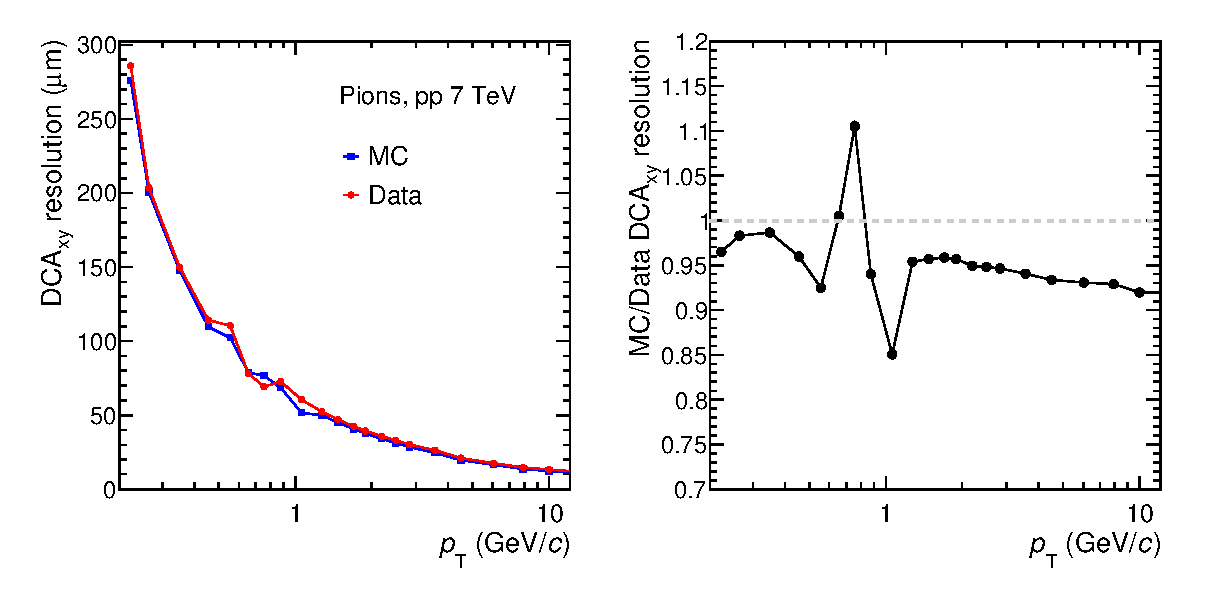
\includegraphics[width=1\textwidth]{FigCap4/DCAxyReso_Pions.eps}
\caption{DCA$_{\rm xy}$ resolution curves of pion tracks as a function of $\pt$ in data and in MC (left panel) and their ratio (right panel) in pp collisions at $\s = 7 $ TeV.}             
\label{fig:DCAxyReso}
\end{center}
\end{figure}
The effect of a variation of the impact parameter resolution in the transverse plane
was also investigated. Fig.~\ref{fig:DCAxyReso} (left) shows, as an example for pion tracks, distributions of
DCA$_{\rm xy}$ resolution as a function of $\pt$ in data and in simulation 
in pp collisions at $\s = 7 $ TeV. The values were extracted via fits to the DCA$_{\rm xy}$ distributions
of tracks in data and in MC, in different $\pt$ intervals, and resulted from the RMS of
such fits. The right panel of the Fig.~\ref{fig:DCAxyReso} shows the 
MC-to-data ratio of DCA$_{\rm xy}$ resolutions. 
The agreement is overall good. To estimate the effect of the residual discrepancy at hight $\pt$,
the resolution values in MC were reduced up to 10\% and the
DCA$_{\rm xy}$ of tracks in MC smeared according to the new resolution.
The variation of the efficiencies resulted less than 3\%, hence
already included in the quoted 7\% from the cut variation study.
\iffalse
\begin{figure}[!htb]
\begin{center}
 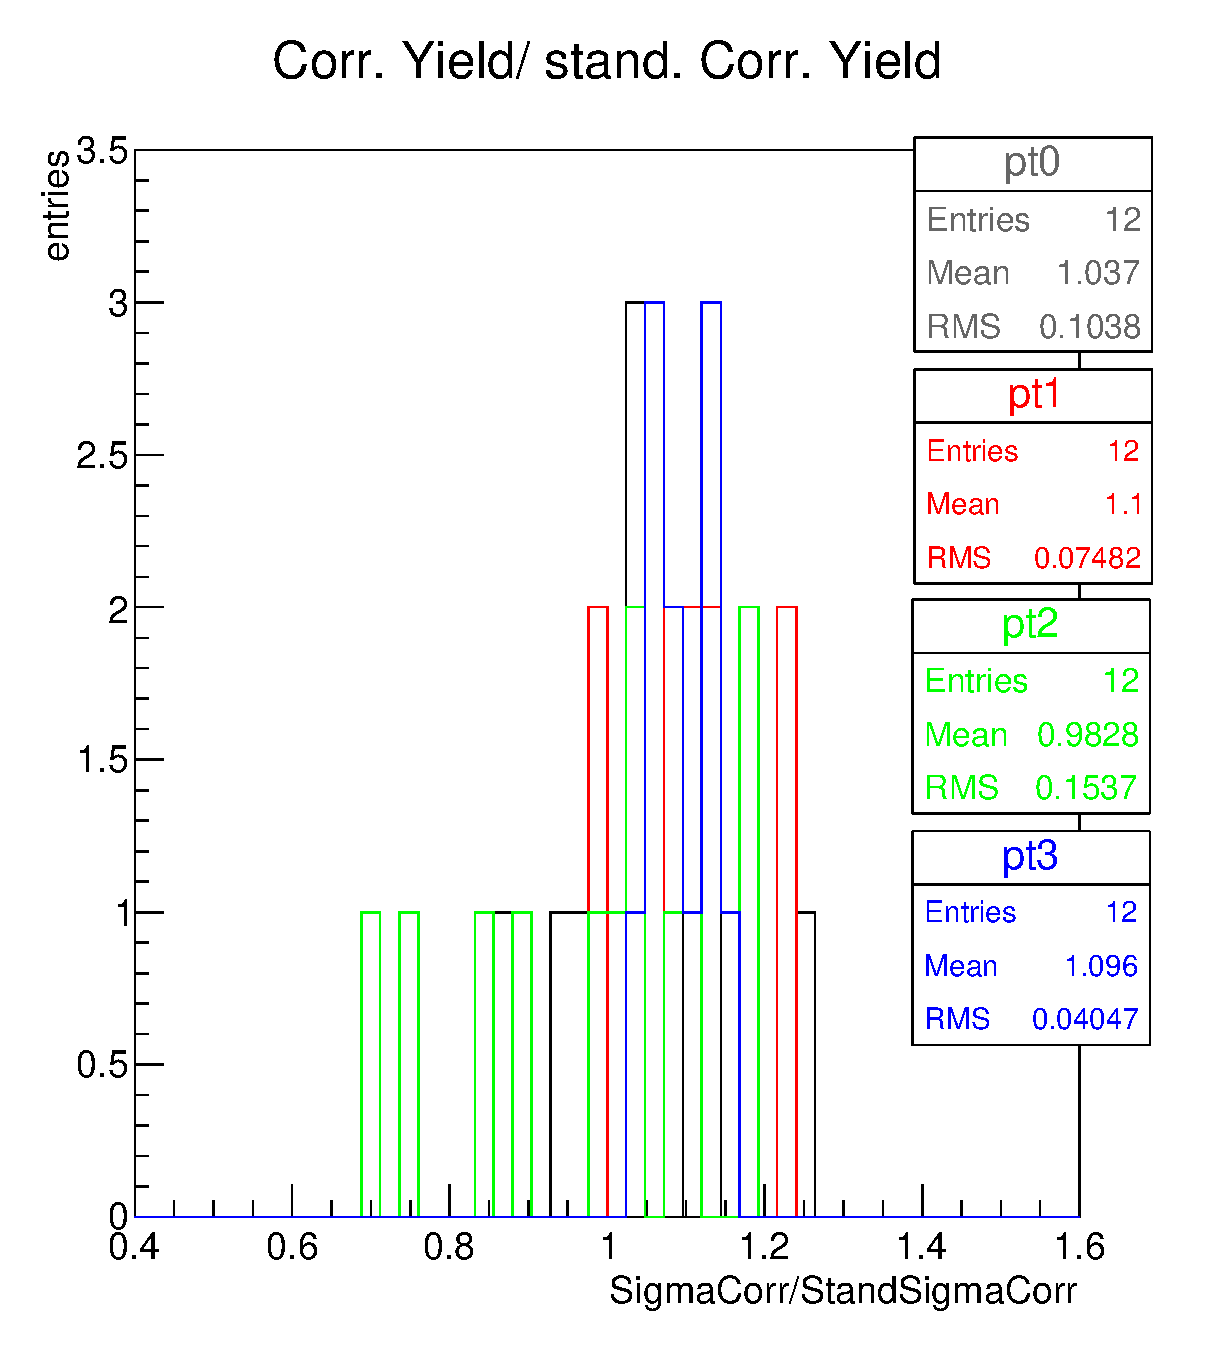
\includegraphics[width=.44\textwidth]{FigCap4/rms_cutvariation.eps}
 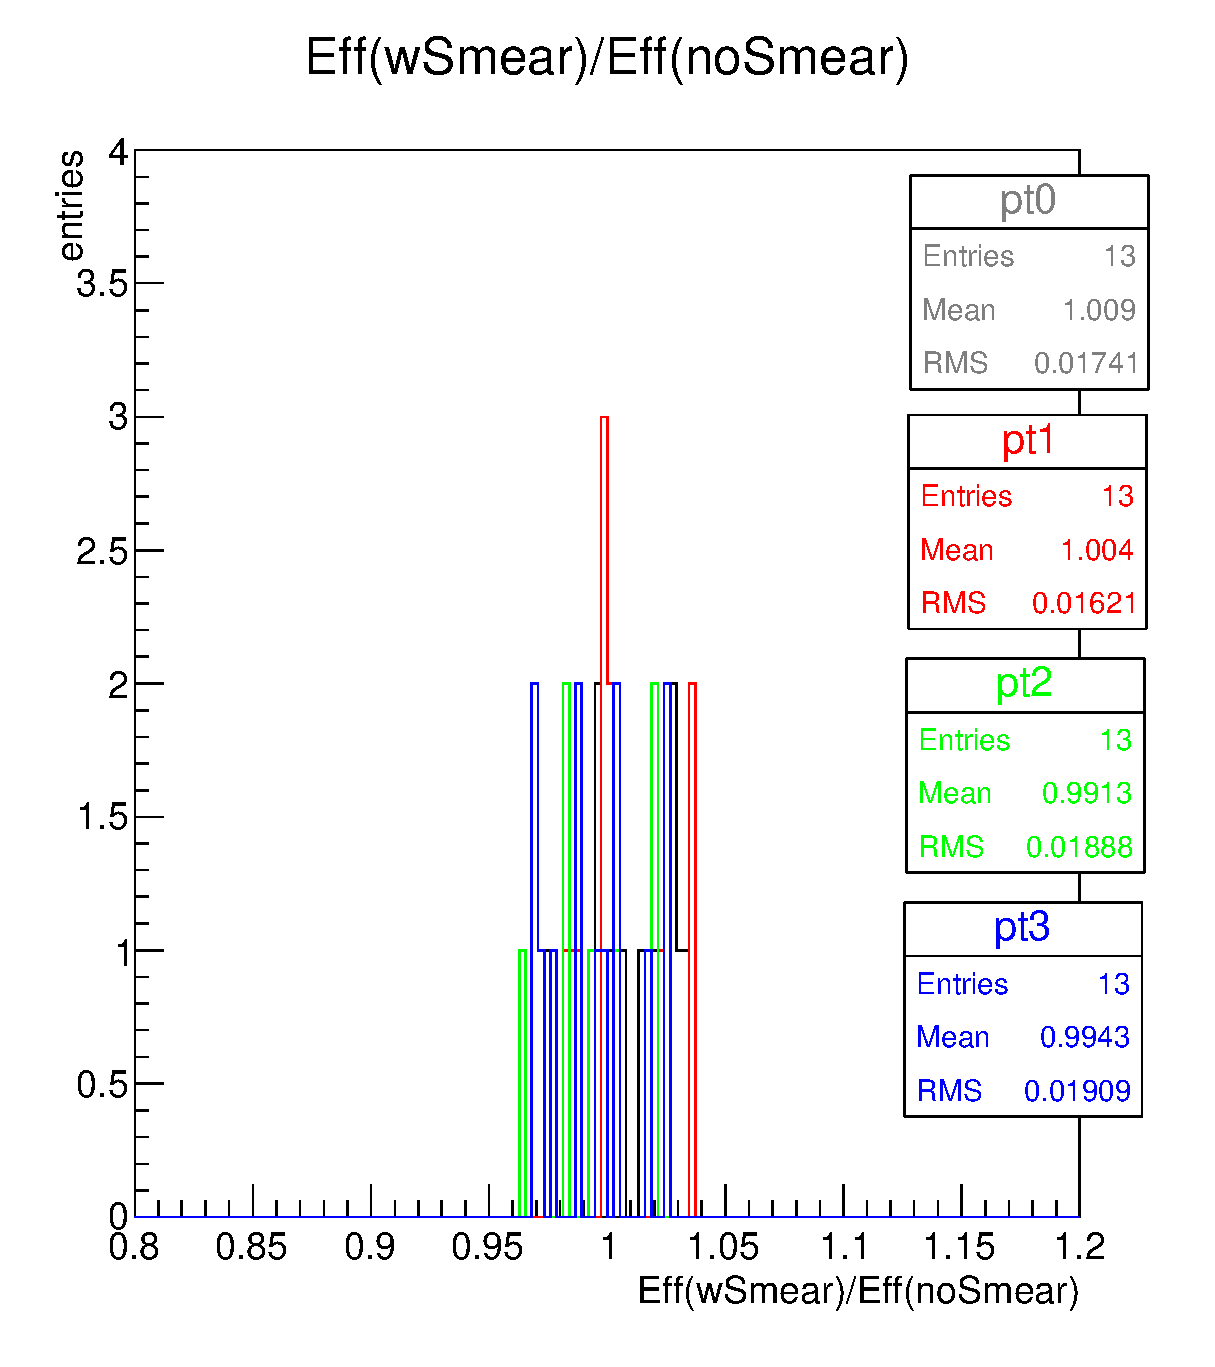
\includegraphics[width=.44\textwidth]{FigCap4/rms_smearp10.eps}
\caption{Left: $\Ds$ corrected yield measured with 12 different sets of
cuts and compared to the yield from the best set of cuts (chosen for the central yield value). Right: ratio for $\Ds$ efficiencies w/o a 
10\% smearing on the xy impact parameter resolution.}             
\label{fig:cutVariation}
\end{center}
\end{figure}
\fi

\subsection{PID efficiency}
\label{sec:PIDsystPP}
To test the efficiency correction of PID selections, a looser PID cut
was used with respect to the default selection described in Sec.~\ref{Sec:PID}. 
In fact, in the $\Ds$ case, the rare signal and the large background 
do not allow for a signal extraction without 
particle identification. The looser PID selection accepts those cases 
reported in Fig.~\ref{fig:strongPID} where combined response values from TPC and TOF 
detectors are 0,1 or 2.
In Fig.~\ref{fig:rmsPID} the ratio
of the corrected yields obtained with looser-to-default PID selection is shown, 
for the twelve different sets of cuts discussed in Sec.~\ref{sec:CutVariation}.
The evaluation of the systematic uncertainty, estimated as the RMS of the distributions in each $\pt$ 
interval, was made considering only the region $\pt > 4 \, \Gevc$, since at lower $\pt$ 
yield extraction with looser PID does not guarantee a statistical significance
of the signal peak larger than 3. The RMS of the yield distributions for the considered
$\pt$ intervals is around 7\% and this value is attributed as uncertainty at all $\pt$.

\begin{figure}[!htb]
\begin{center}
 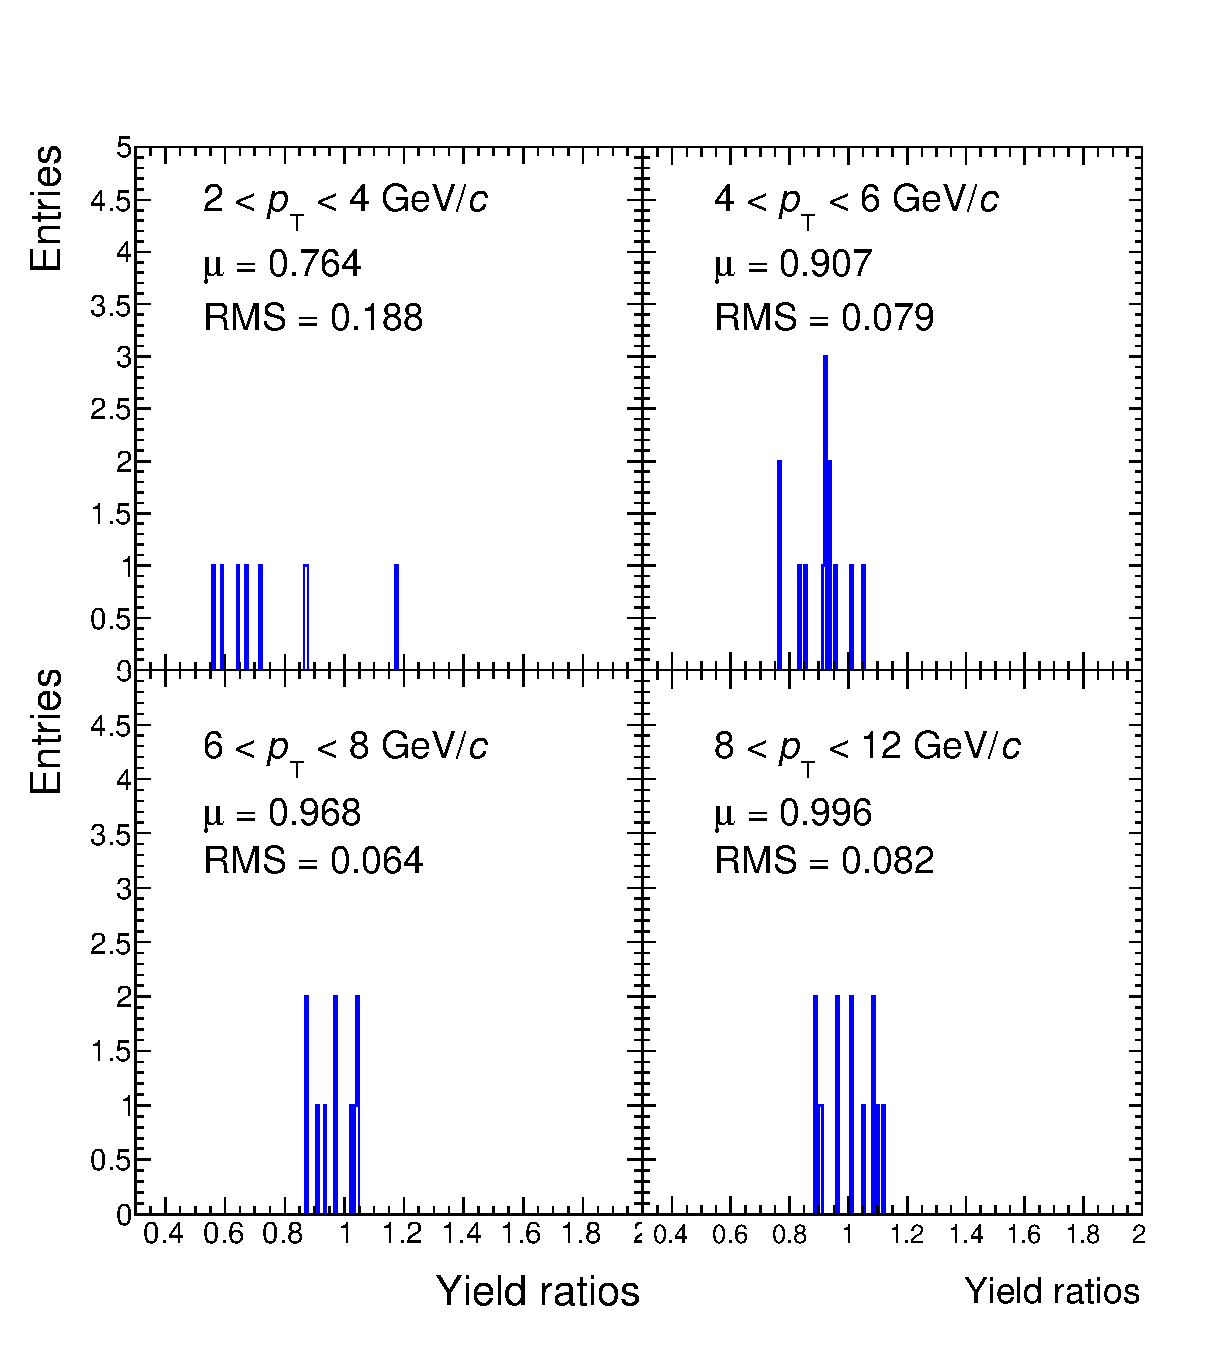
\includegraphics[width=.7\textwidth]{FigCap4/PIDrms4x4}
\caption{Ratio of $\Ds$ corrected yields with looser and default PID selections (for twelve different sets of
topological selections).}
\label{fig:rmsPID}
\end{center}
\end{figure}

\subsection{Track reconstruction efficiency}
\label{sec:TrackEffSystPP}
The systematic uncertainty related to the tracking efficiency includes the 
effects arising from track finding in the TPC, from track prolongation  
from the TPC to the ITS, and from track quality selections.
It was estimated with the following tests:
\begin{itemize}
\item comparison of the D-meson cross sections obtained with different track selection cuts;
\item comparison of the TPC-ITS track matching efficiency in data and simulations.
\end{itemize}
These checks are discussed in the following subsections.

\subsubsection{Variation of track selections}
For this purpose, $\Dzero$ and $\Dplus$ mesons were used due to their
higher statistical significance of the extracted yields.
The D-meson raw yields and efficiencies were evaluated with 
different sets of track selection cuts.
The following selections were tested:
\begin{enumerate}
\item additional cut on number TPC crossed rows $> 120-(5/\pt)$;
\item additional number of TPC clusters $>0.65 \times$ number of TPC crossed rows;
\item ratio of crossed rows over findable clusters in the TPC $>0.9$.
\end{enumerate}
The systematic uncertainty was assigned based on the observed variation of
the prompt $\Dzero$ and $\Dplus$ cross sections with respect to the default selections.
Based on this check systematic uncertainties of 2\% and 3\% were 
respectively estimated for $\Dzero$ (two-body decay) and $\Dplus$ (three-body decay) 
due to variation of track cuts. The values are consistent with a 1\% per-track systematic
uncertainty.

\subsubsection{ITS-TPC matching efficiency}

Matching efficiency, i.e. efficiency of track prolongation from TPC to ITS, 
is defined as the fraction of tracks with 
clusters in both ITS and TPC over the number of tracks with clusters in TPC.
Systematic uncertainty on its determination arises from discrepancies 
in efficiency between data and Monte Carlo.
Matching efficiency for primary tracks is expected to be higher than 
for secondary tracks (originating from strangeness decay, thus 
with secondary vertices likely to be out of SPD or for tracks arising
 from interaction with material).
If the fractions of primary and secondary tracks are different in data 
and in Monte Carlo, this could lead to a wrong estimation of the systematic 
uncertainty in the matching. Hence, the idea of this study is to 
use data-driven corrections of primary and secondary fractions to weight the MC
and obtain a corrected inclusive MC efficiency. The latter will be compared 
with efficiency on data to extract the systematic uncertainty.\\
The ingredients are:
\begin{itemize}
\item matching efficiencies for different particle types: 
Eff$^{\rm MC}_{\rm primaries}$, Eff$^{\rm MC}_{\rm secondaries}$, Eff$^{\rm Data}_{\rm inclusive}$
\item fraction of primary tracks in data: f'$_{\rm primaries}$
\item corrected MC-inclusive efficiency: 
Eff$^{\rm MC}_{\rm inclusive}$ = f'$_{\rm primaries}$ x Eff$^{\rm MC}_{\rm primaries}$ + (1- f'$_{\rm primaries}$) x Eff$^{\rm MC}_{\rm secondaries}$
\item systematic uncertainty: 
(Eff$^{\rm Data}_{\rm inclusive}$ - Eff$^{\rm MC}_{\rm inclusive}$)/Eff$^{\rm Data}_{\rm inclusive}$.
\end{itemize}
A minimum-bias Monte Carlo production anchored to 2010 pp data taking at 
$\s = 7$ TeV was used. Charm-enriched productions were not used in this study 
since the shape of DCA distribution of tracks (used to extract data-driven 
primary track fraction) is affected by the heavy-flavour enhancement
and may bias the fit.
Efficiency was studied as a function of:
\begin{itemize}
\item $\pt$, from 0.5 to 15 $\Gevc$
\item $\phi$, between (0,2$\pi$)
\item $\eta$, between (-0.8,0.8)
\end{itemize}

Let's examine below more in detail the steps needed to 
calculate the systematic uncertainty.
\begin{enumerate}
\item {\bf ITS-TPC matching efficiency:} calculated separately for 
primary and secondary tracks in MC, inclusively on data. For 
the numerator of the efficiency, tracks were selected requiring 
to have a hit in one of the two SPD layers, 
$|$DCAxy$|<$ 2.4 cm and $|$DCAz$|<$ 3.2 cm.
\begin{figure}[!htb]
\centering
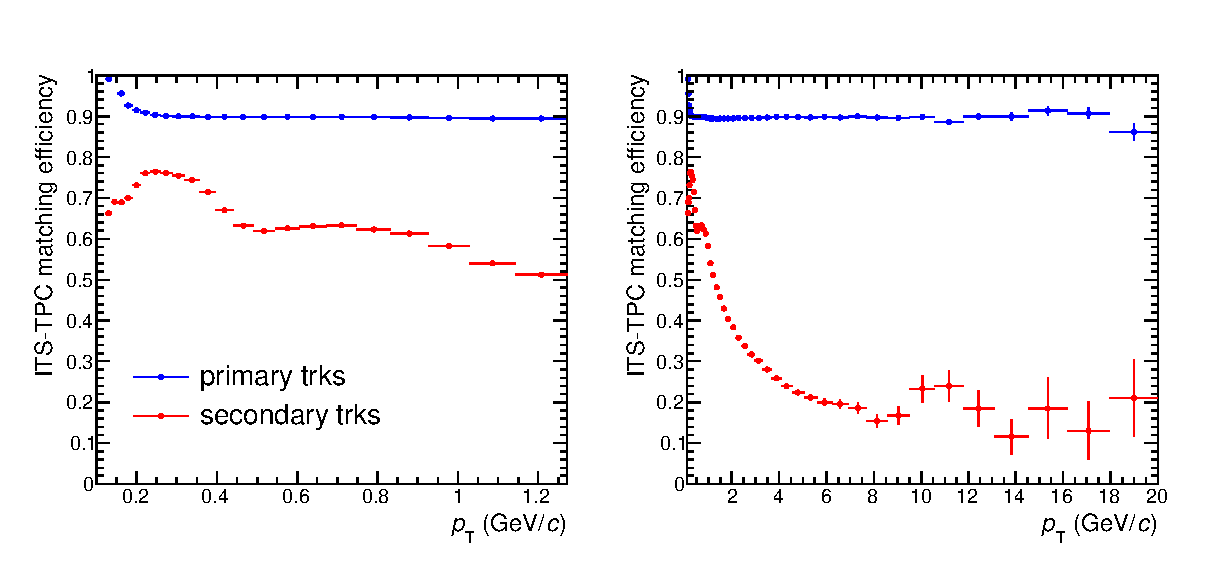
\includegraphics[width=1\textwidth]{FigCap4/ITSTPC_matchEff_vsPt_LowFullpt.eps}
\caption{Matching efficiency for primaries and secondaries tracks as a function of $\pt$ in MC for $\pt$ interval from 0.1 to 1 $\Gevc$ (left) and up to 20 $\Gevc$ (righ). }
\label{fig:matcheff_pt}
\end{figure}

In Fig.~\ref{fig:matcheff_pt}, ITS-TPC matching efficiency 
of charged tracks in MC as a function of 
$\pt$ is shown. The left panel is referred to the low $\pt$ region (0.1-1 $\Gevc$), 
the right one up to 20 $\Gevc$. 

\item {\bf Fractions of primary tracks:} extracted from a fit to
 the track impact parameter distribution in data using MC templates for 
 DCA$_{\rm xy}$ distributions of primary and secondary tracks. The ROOT TFractionFitter 
 package was used to perform the fit. The fit could be resolved 
 using three templates describing primary tracks, secondaries tracks
 from strangeness decay and tracks from interaction with material. 
 A selection on tracks requiring at least one hit in the two SPD layers 
 was used, to assure enough resolution to distinguish primary and 
 secondary DCA$_{\rm xy}$ distributions.
\begin{figure}[!htb]
\begin{center}
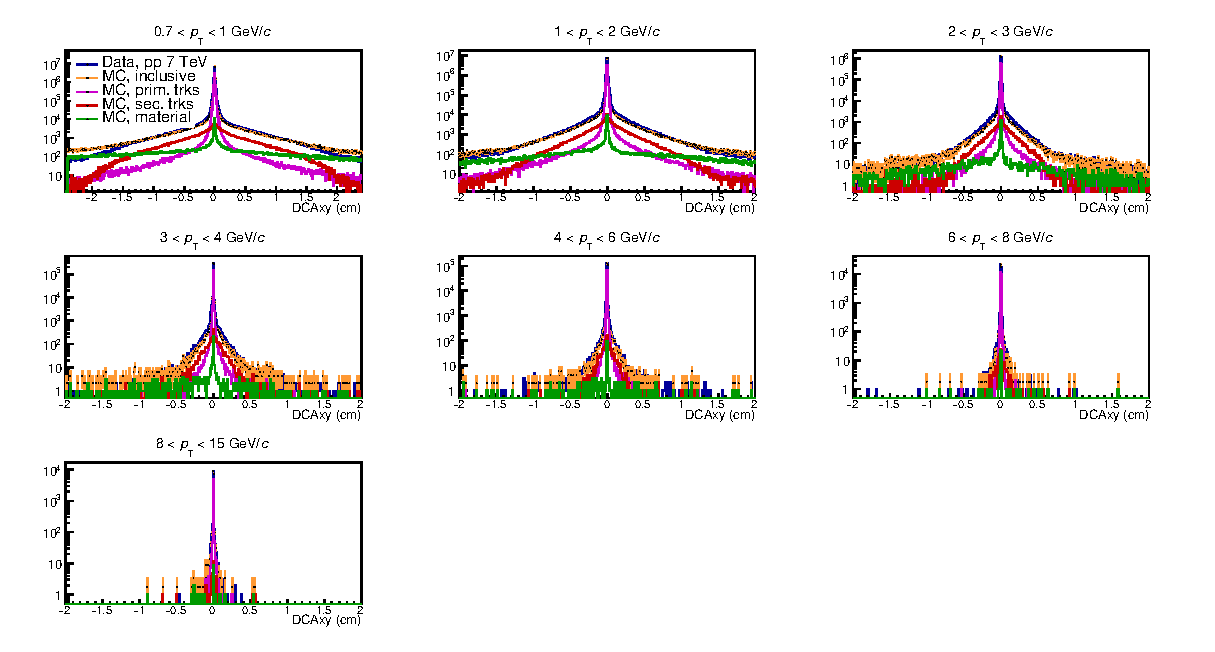
\includegraphics[width=.99\textwidth]{FigCap4/FitComponents.eps}
\caption{DCA$_{\rm xy}$ distributions in data and in MC for primary and secondary tracks in different colours, in $\pt$ intervals from 0.5 to 15 $\Gevc$.}
\label{fig:DCAxyDataMCVsPt}
\end{center}
\end{figure}
\begin{figure}[!hb]
\begin{center}
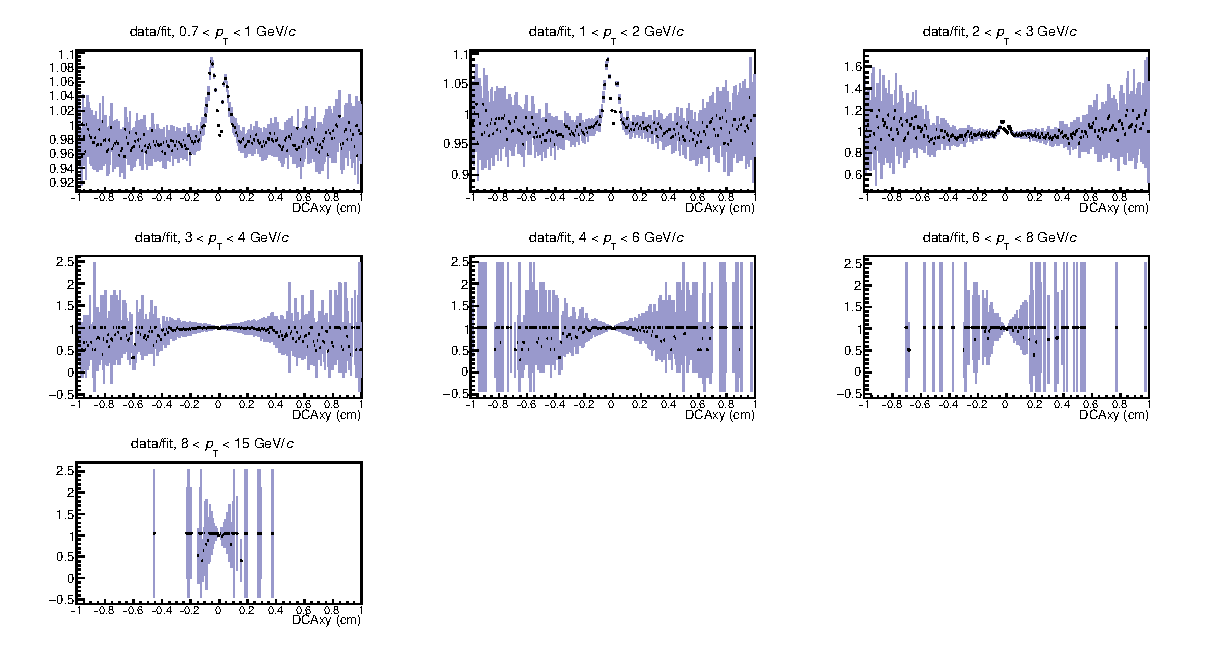
\includegraphics[width=.99\textwidth]{FigCap4/DataOverFit.eps}
\caption{Ratio of DCAxy distributions in data and in the fit result histograms, in $\pt$ intervals from 0.5 to 15 $\Gevc$.}
\label{fig:DCAxyRatioDataFitVsPt}
\end{center}
\end{figure}
Fits were performed on the DCA$_{\rm xy}$ distributions of charged particles 
in the range [-1,1] cm, in different intervals of $\pt$, $\phi$, $\eta$ 
and constraining the three fractions within reasonable minimum and maximum values.
The fractions were then calculated by integrating the histogram 
resulting from the fit in the range $|$DCA$_{\rm xy}|<$ 2.4 cm, for
consistency with what done for matching efficiency calculation. 
As a closure test, it was verified that the MC values for fractions of primary and secondary tracks 
were in agreement with the values extracted when performing the fit with TFractionFitter 
on the inclusive MC distribution (instead of data), with the three MC templates.  
In Fig.~\ref{fig:DCAxyDataMCVsPt} the distributions of DCA$_{\rm xy}$ 
in data and in MC for the different components are
shown in different colours, in $\pt$ intervals from 0.5 to 15 $\Gevc$. 
In Fig.~\ref{fig:DCAxyRatioDataFitVsPt} the ratio of DCA$_{\rm xy}$ distributions 
in data to the distribution resulting from the fit are plotted. 
Finally, in Fig.~\ref{fig:Fractions}, the data-driven values of primary and secondary
 fractions are shown and compared to 
 the ones obtained from original values in MC (empty markers). 
The fraction of secondaries in the figure already includes contribution 
from material. We conclude that the fraction of secondaries is underestimated in MC.
\begin{figure}[!hb]
\begin{center}
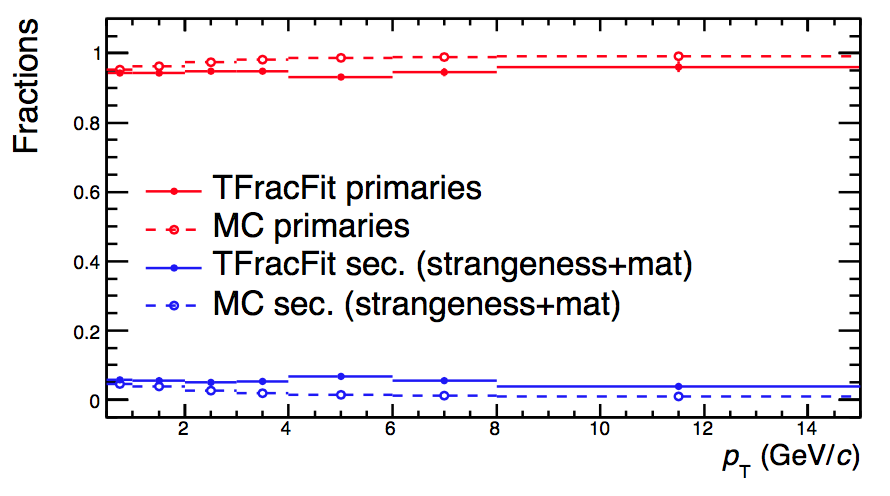
\includegraphics[width=.6\textwidth]{FigCap4/MEfractions.png}
\caption{Data-driven (solid lines) and MC original (dashed lines) fractions of primary (red) and secondary (blue) tracks as a function of $\pt$ in pp collisions at $\s = $ 7 TeV.}
\label{fig:Fractions}
\end{center}
\end{figure}

\item {\bf Correction to the primary fraction:} since the fraction of primary
 particles was calculated using tracks with the request of a hit in one of the SPD layers, 
the primary fraction of this sample 
needs to be rescaled to the primary fraction of the sample of tracks in the TPC. 
The correction factor is based on MC information and obtained as 
the ratio of the fraction of primary tracks in TPC to the fraction of primary
 tracks with TPC-ITS matching. The final fraction of primary tracks is hence
  f'$_{\rm primaries}$ = f$_{\rm primaries}$ x correction factor, 
  where f$_{\rm primaries}$ is the fraction obtained at step 2. 
  Typical values of correction factor for primary tracks are around $\sim$ 0.95-0.98. 
  In Fig.~\ref{fig:MCfractions} an example of fractions of primary 
  and secondary tracks in MC requiring ITS-TPC matching or points in the TPC detector only are 
  shown in different colours as a function of $\pt$.
\begin{figure}[!htb]
\begin{center}
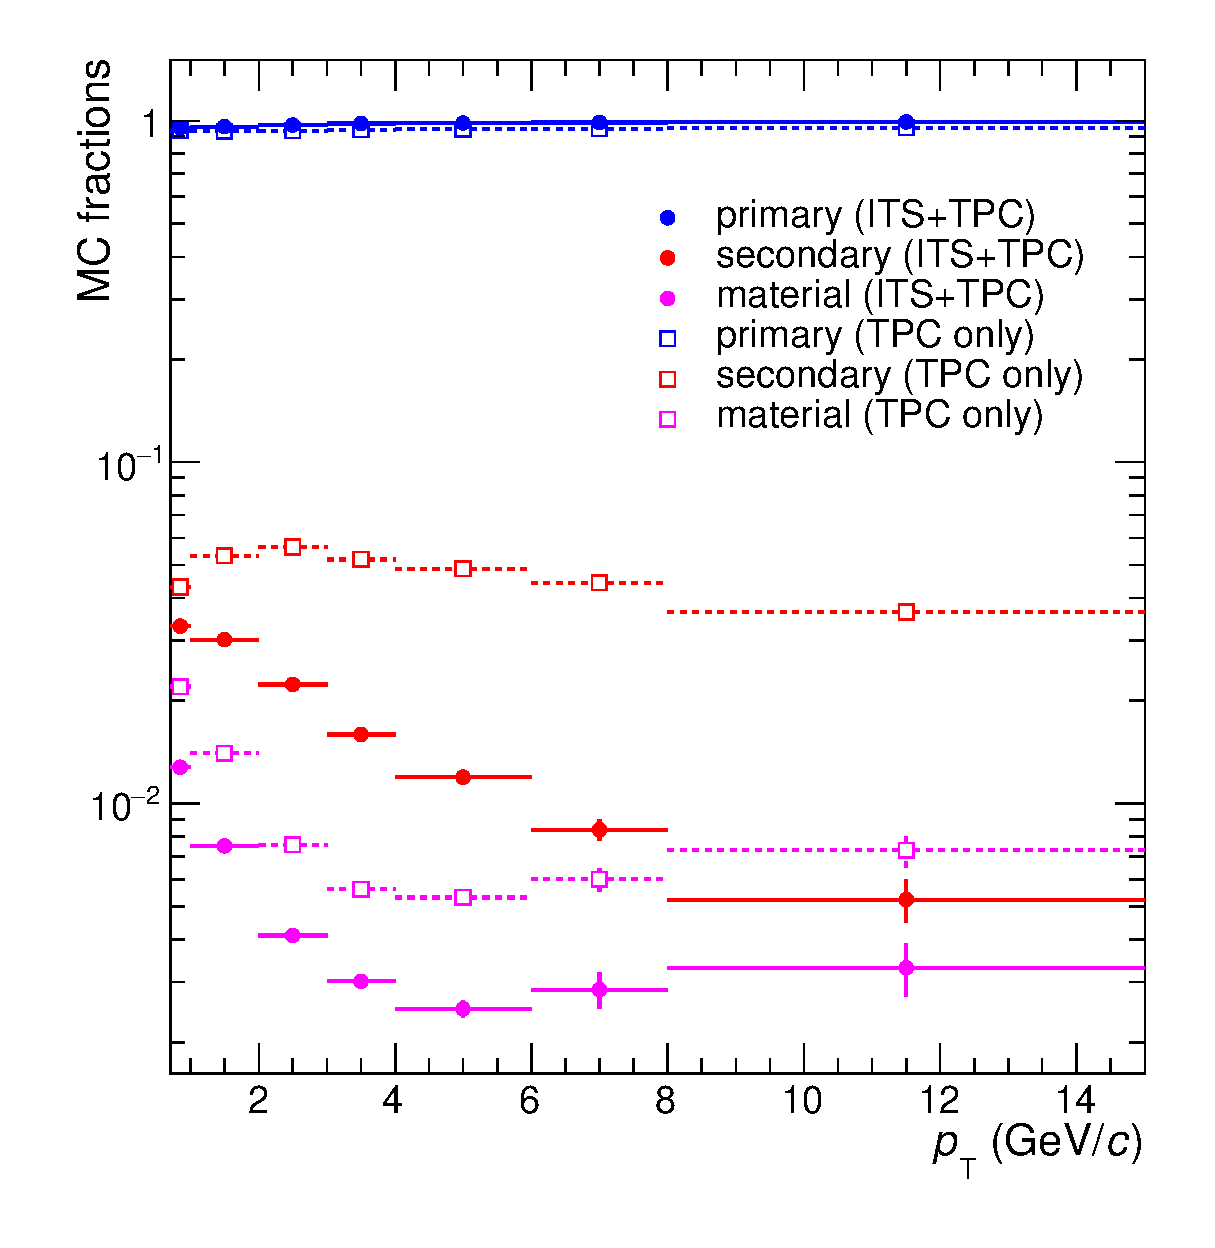
\includegraphics[width=.50\textwidth]{FigCap4/MCfractions_ESDTrOnly_VsPt_PiK.eps}
\caption{Example of fractions of primary and secondary tracks in MC requiring ITS-TPC or TPC only in different colours as a function of $\pt$.}
\label{fig:MCfractions}
\end{center}
\end{figure}

\item {\bf ITS-TPC corrected matching efficiency:} calculated 
as  Eff$^{\rm MC}_{\rm inclusive}$ = f'$_{\rm primaries}$ x Eff$^{\rm MC}_{\rm primaries}$ + (1- f'$_{\rm primaries}$) x Eff$^{\rm MC}_{\rm secondaries}$. The corrected matching efficiency 
is shown in Fig.~\ref{fig:CorrMatchEffVsPt},~\ref{fig:CorrMatchEffVsPhi} 
(left) and~\ref{fig:CorrMatchEffVsEta} (left)
as a function of $\pt$, $\phi$, $\eta$ respectively, for kaons and 
pions (requiring a 3$\sigma$ PID cut in TPC). 
It was verified that no substantial changes are obtained if 
considering all the species ($\pi, {\rm K}, p, e, \mu$). 
The drops in efficiency at some $\phi$ regions are due to SPD
inefficiencies during the data taking.
Finally, the ratios of MC inclusive corrected efficiencies to
efficiency in data are shown in Fig.~\ref{fig:MatchEffSystVsPt},~\ref{fig:CorrMatchEffVsPhi} 
(right) and~\ref{fig:CorrMatchEffVsEta} (right) as a function of 
$\pt$, $\phi$, $\eta$ respectively. The data driven weighting procedure 
in MC allows to quote a truthful and reduced systematic uncertainty
especially as a function of $\pt$. 
\begin{figure}[!htb]
\begin{center}
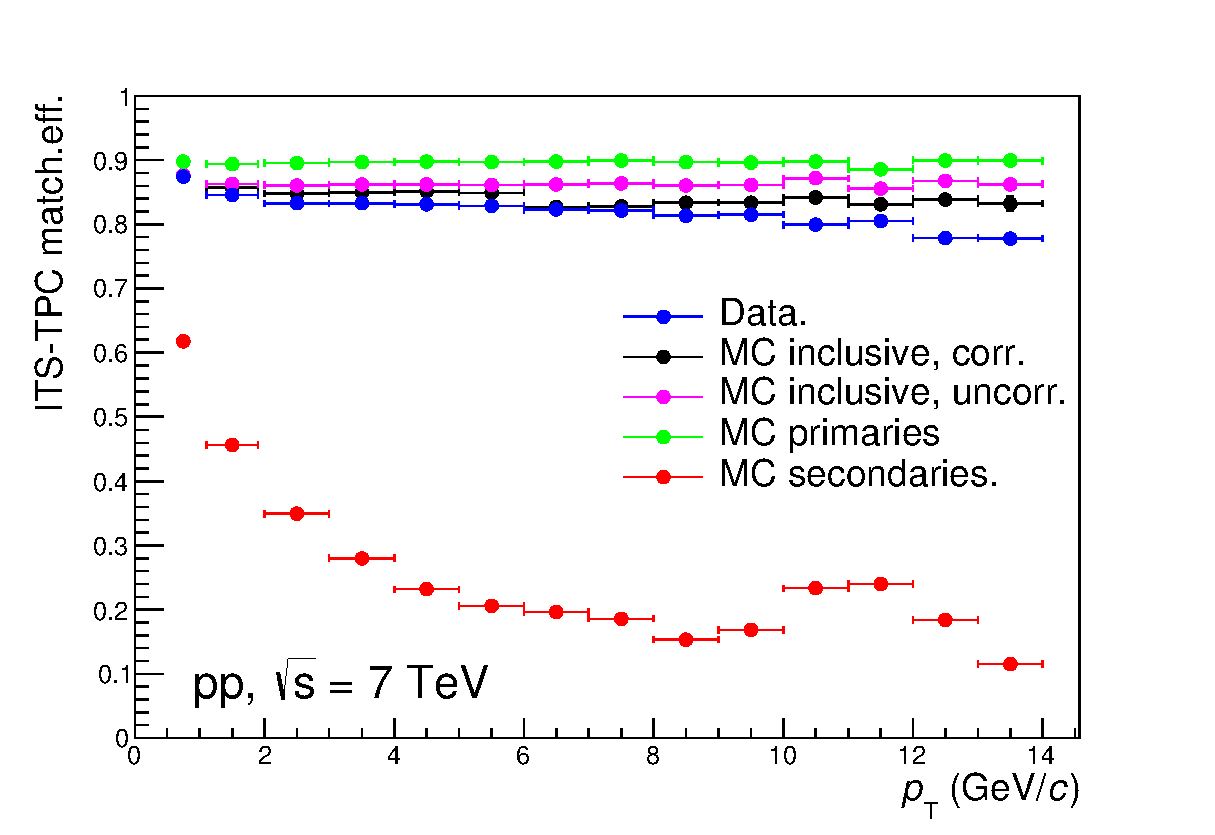
\includegraphics[height=7cm]{FigCap4/ITSTPCmatchEff_10bpass4_vsPt.eps}
\caption{ITS-TPC matching efficiency as a function of $\pt$ for 2010 pp data taking at $\s = 7$ TeV. The matching efficiency is shown for data (blu), for MC primary (green) and secondary (from strangeness decay and material interaction, in red) tracks, for inclusive MC tracks with (black) and without (magenta) data-driven correction. }
\label{fig:CorrMatchEffVsPt}
\end{center}
\end{figure}
\begin{figure}[!htb]
\begin{center}
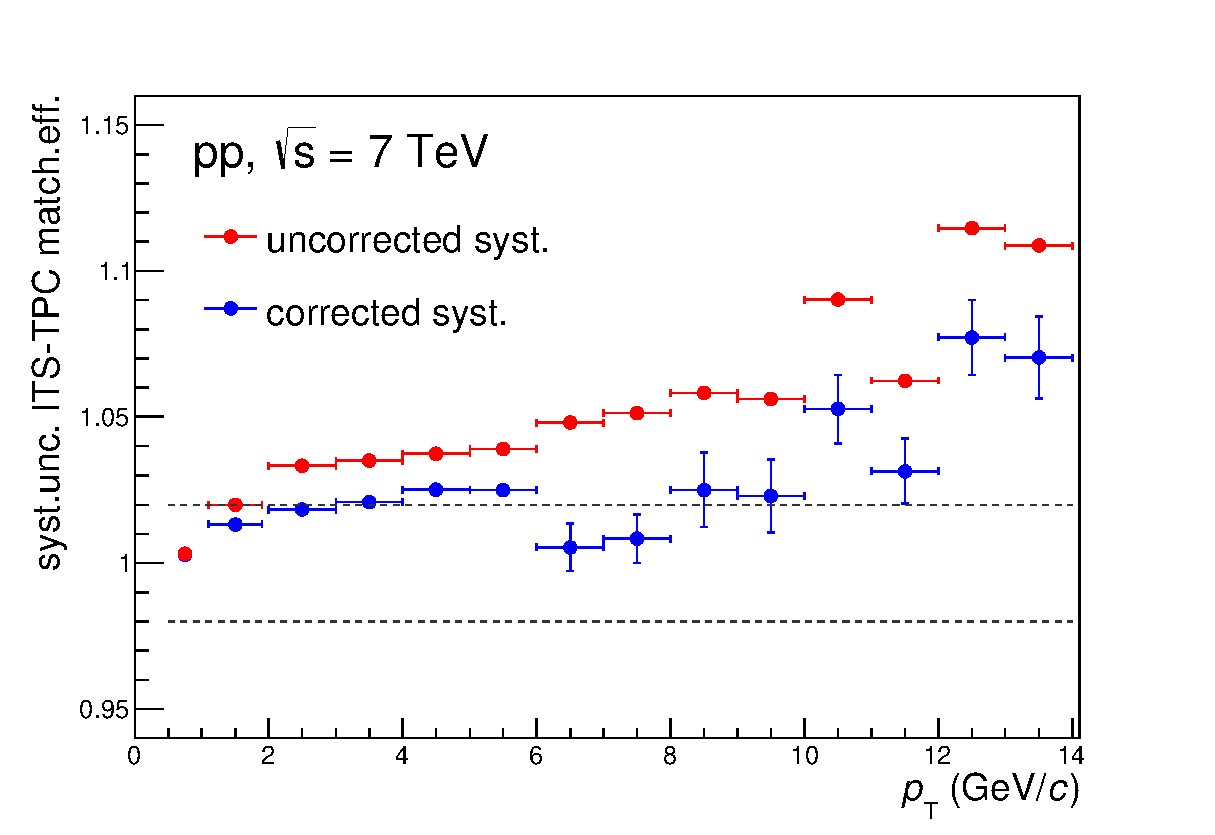
\includegraphics[height=7cm]{FigCap4/ITSTPCmatchEffSyst_10bpass4_vsPt.eps}
\caption{ITS-TPC matching efficiency systematics as a function of $\pt$ before (red) and after (blue) data-driven correction.}
\label{fig:MatchEffSystVsPt}
\end{center}
\end{figure}
A final systematic uncertainty of 2\% per track was assigned for particles 
between 2-6 $\Gevc$, and of 1\% at lower and higher $\pt$.
This per-track uncertainty is then summed in quadrature with the 
1\% per-track systematic uncertainty on track selection. 
{\bf Qui devo ricontrollare: con gli output che ho per il 10bpass4, non riesco ad ottenere
gli stessi valori (leggeremente piu' piccoli) per la ME che avevamo usato per il paper. Mi ricordo che ad un certo punto avevamo rigirato sul pass4 dopo che avevamo scoperto un baco: non e' molta la differenza appunto, ma non torna con i plot 4.21 specialmente ad alto pt... Non so se val la pena rimandare dei jobs per rifare il plot 4.21 ed essere coerenti qui.}
\end{enumerate}
Finally, a MC simulation was used to propagate the uncertainty at the 
track level to the D-meson level through the daughter's 
kinematic. In the simulation the same topological and PID cuts used in data were 
applied. In the left column of Fig.~\ref{fig:SysMatchEffDmeson}, the scatter plots of 
$\pt$  of daughter tracks versus 
D-meson $\pt$ (for $\Dplus$, $\Ds$, $\Dzero$ and $\Dstar$ from top to bottom) are presented. 
The right column shows the final systematic uncertainty of tracking 
efficiency for 2- and 3-prong D mesons as a function of $\pt$, propagated via
daughter track kinematics.

\begin{figure}[!htb]
\begin{center}
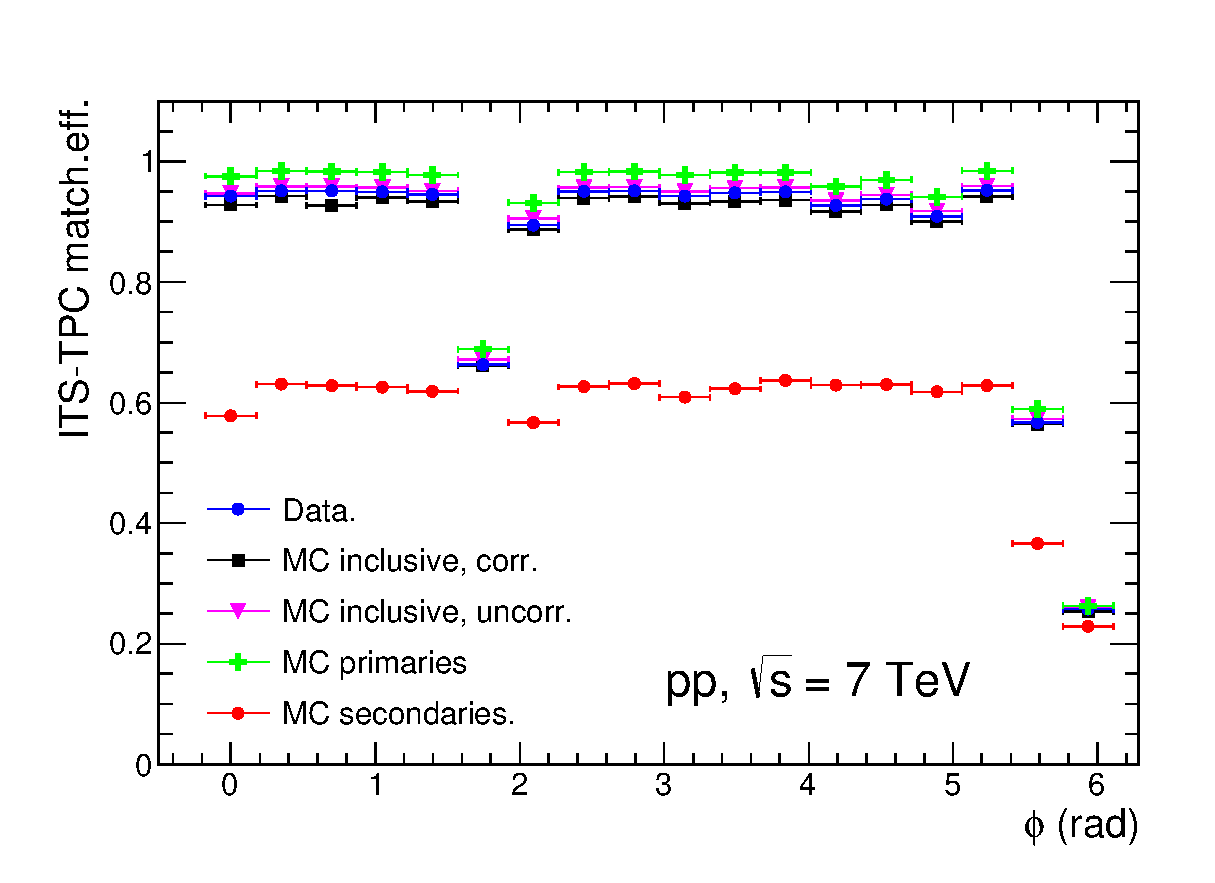
\includegraphics[width=.49\textwidth]{FigCap4/ITSTPCmatchEff_10bpass4_vsPhi.eps}
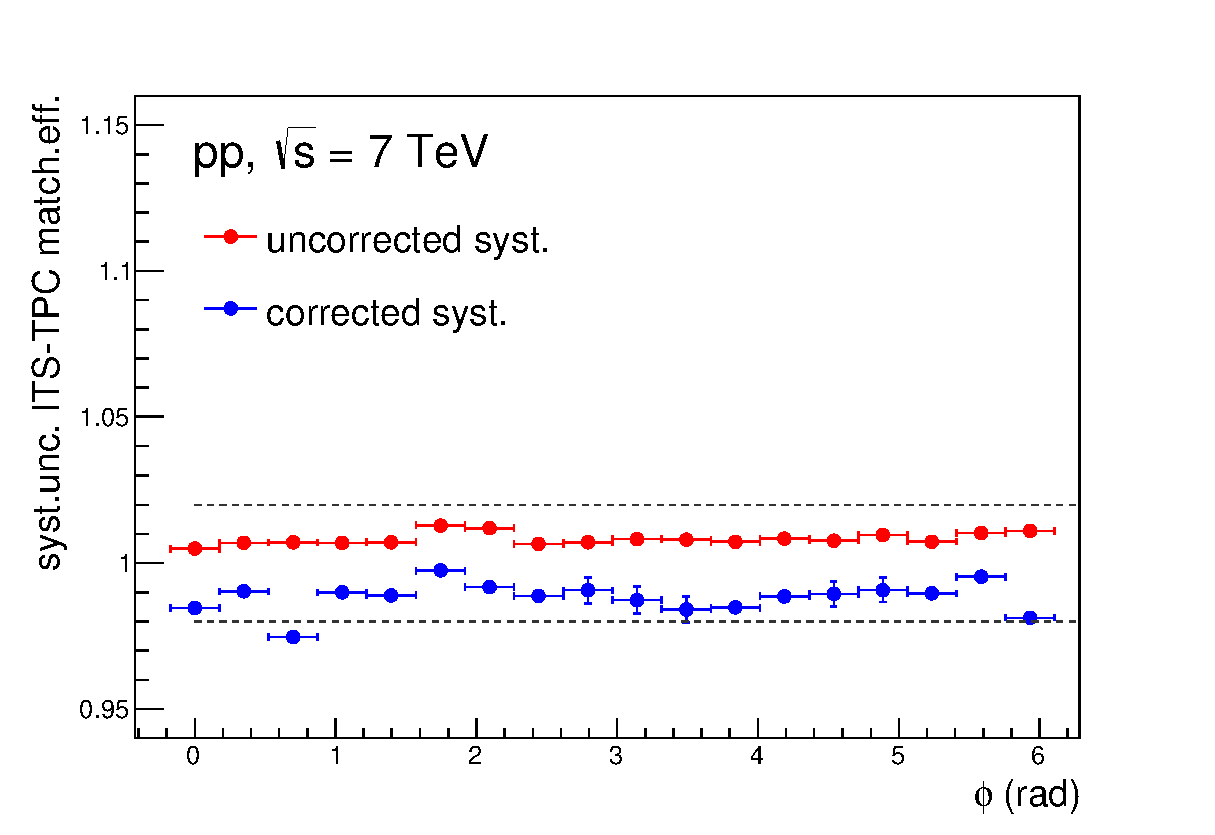
\includegraphics[width=.49\textwidth]{FigCap4/ITSTPCmatchEffSyst_10bpass4_vsPhi.eps}
\caption{Left: ITS-TPC matching efficiency as a function of $\phi$ for 2010 pp data taking at $\s = 7$ TeV. The matching efficiency is shown for data (blu), for MC primary (green) and secondary (from strangeness decay and material interaction, in red) tracks, for inclusive MC tracks with (black) and without (magenta) data-driven correction. Right: ITS-TPC matching efficiency systematics as a function of $\phi$ before (red) and after (blue) data-driven correction.}
\label{fig:CorrMatchEffVsPhi}
\end{center}
\end{figure}

\begin{figure}[!htb]
\begin{center}
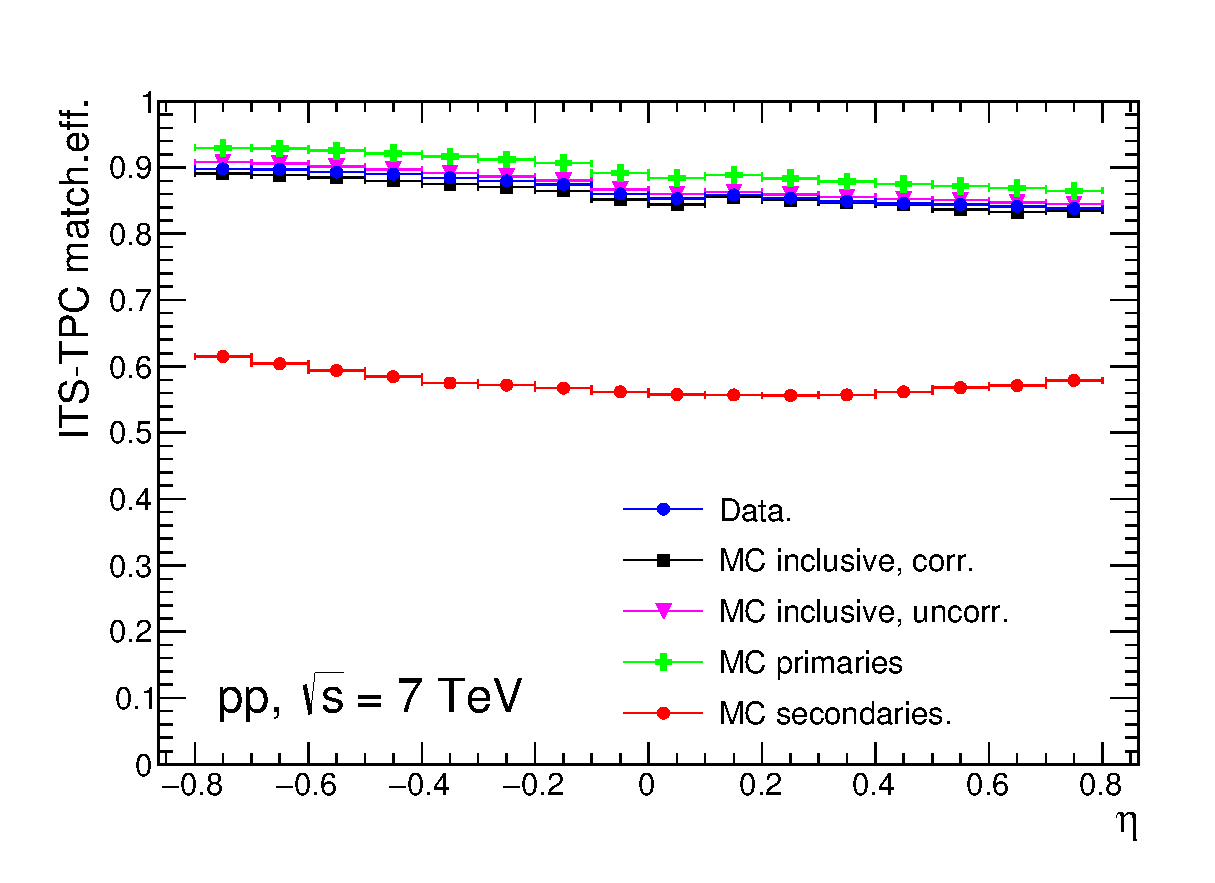
\includegraphics[width=.49\textwidth]{FigCap4/ITSTPCmatchEff_10bpass4_vsEta.eps}
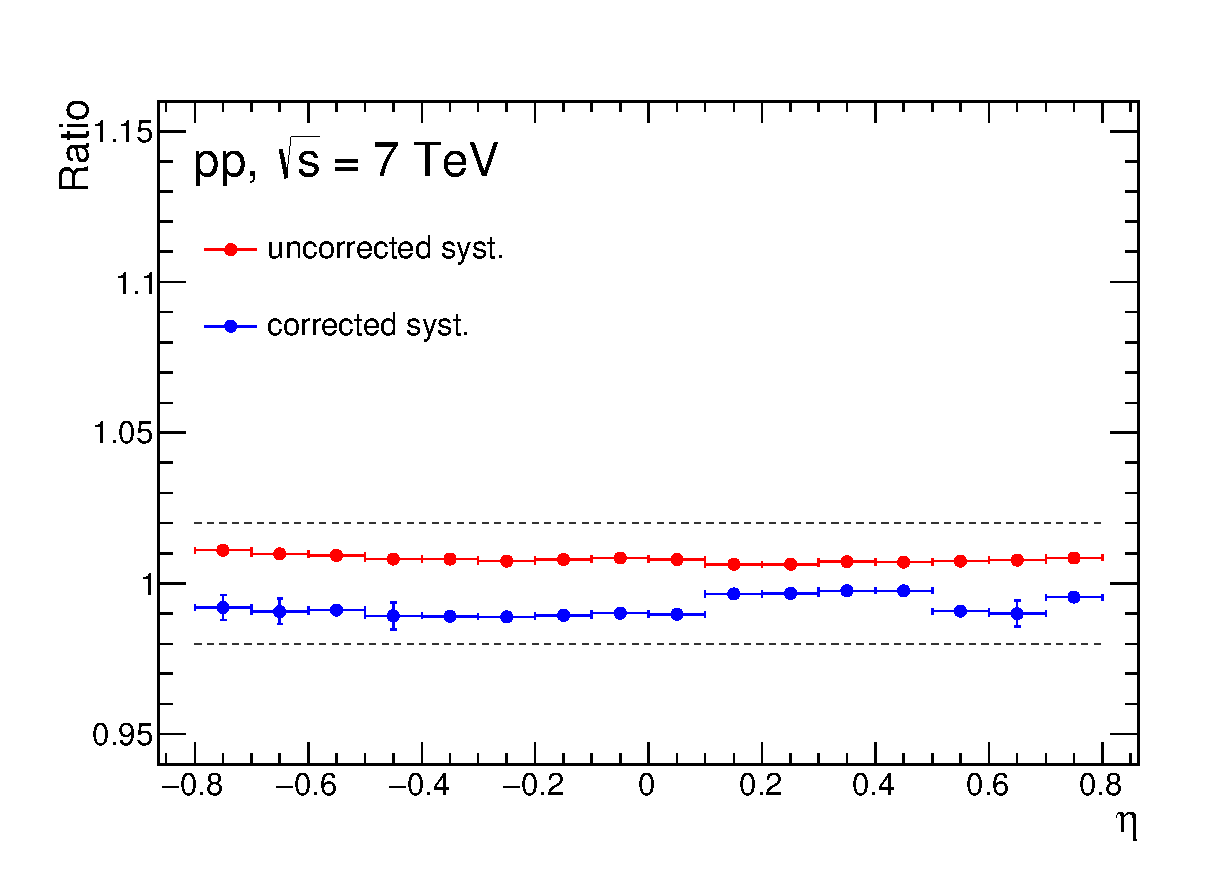
\includegraphics[width=.49\textwidth]{FigCap4/ITSTPCmatchEffSyst_10bpass4_vsEta.eps}
\caption{Left: ITS-TPC matching efficiency as a function of $\eta$ for 2010 pp data taking at $\s = 7$ TeV. The matching efficiency is shown for data (blu), for MC primary (green) and secondary (from strangeness decay and material interaction, in red) tracks, for inclusive MC tracks with (black) and without (magenta) data-driven correction. Right: ITS-TPC matching efficiency systematics as a function of $\eta$ before (red) and after (blue) data-driven correction.}
\label{fig:CorrMatchEffVsEta}
\end{center}
\end{figure}


\begin{figure}[!htb]
\begin{center}
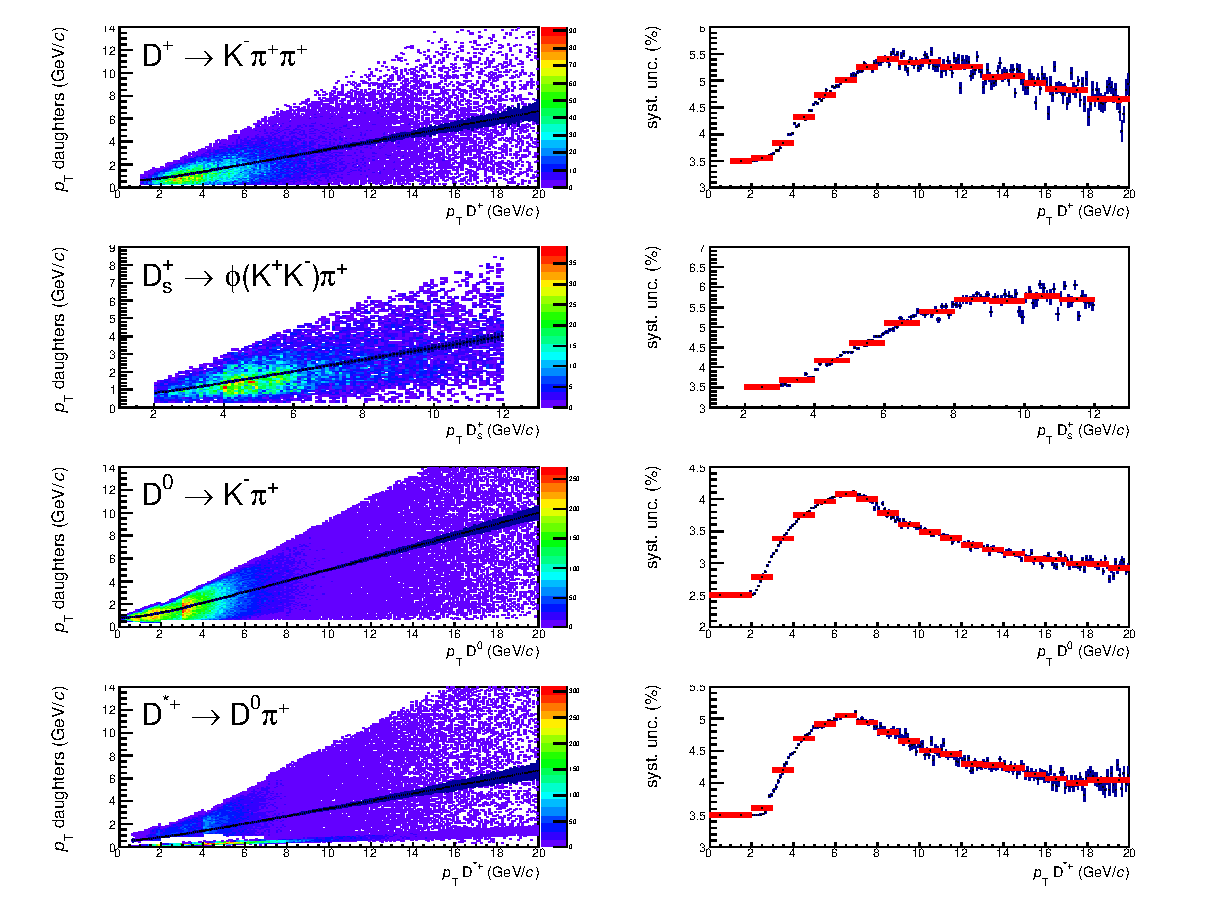
\includegraphics[width=1\textwidth]{FigCap4/FinalSystMEDmesons_ppPass4.eps}
\caption{Left column: scatter plot of daughter's $\pt$ versus D-meson $\pt$ for $\Dplus$, $\Ds$, $\Dzero$ and $\Dstar$ from top to bottom. Right column: final systematic uncertainties propagated at D-meson level after weighting for daughter's kinematics, as a function of $\pt$.}
\label{fig:SysMatchEffDmeson}
\end{center}
\end{figure}

\subsection{B feed-down}
\label{sec:BfdSub}
The systematic uncertainty on the subtraction of feed-down component from 
beauty-hadron decay was estimated by varying the $\pt$-differential 
cross section of feed-down D mesons within the theoretical uncertainties
of the FONLL calculation. The procedure for the variation of the $b$-quark mass, 
of the perturbative scales and of the parton distribution functions is described 
in~\cite{Cacciari:2012ny}. The uncertainty related to the B decay 
kinematics was disregarded, after verifying that the difference resulting 
from using the PYTHIA~\cite{Sjostrand:2006za} decayer instead of 
EvtGen~\cite{Lange:2001uf} is negligible 
with respect to the FONLL B-meson cross-section uncertainty.
Previous D-meson analyses in 
ALICE~\cite{ALICE:2011aa,Abelev:2012tca,Adam:2016ich,Adam:2015jda} 
used to compare two different methods for the subtraction of the beauty feed-down component 
and include their difference in this systematic uncertainty. 
The first method, used to give the central value for $f_{\rm prompt}$, 
is presented in Eq.~\ref{eq:fpr} and needs as inputs FONLL predictions
of B-meson cross-sections and selection efficiency for B feed-down 
D mesons. The alternative method takes as inputs FONLL predictions for both 
feed-down and prompt D mesons and their respective Monte Carlo efficiencies, 
as follows:
\begin{equation}
f^\prime_{\rm prompt} = \left( 	1 + 	\frac{({\rm Acc}\times\epsilon)_{{\rm feed-down}}}{({\rm Acc}\times\epsilon)_{{\rm prompt}}}	\cdot
		 \frac{ \left(\frac{{\rm d}^2 \sigma}{{\rm d}y \, {\rm d} \pt } \right)^{{\sf FONLL}}_{{\rm feed-down}} }{ \left(\frac{{\rm d}^2 \sigma}{{\rm d}y \, {\rm d} \pt } \right)^{{\sf FONLL}}_{ {\rm prompt} } } 
\right)^{-1} \, .
\label{eq:fc}
\end{equation}
A review of currently available measurements of beauty and 
charmed meson cross-sections at the LHC was carried out. The measurements 
were compared to FONLL predictions for heavy-flavoured hadrons 
for the specific center-of-mass energy and rapidity interval.
In Fig.~\ref{fig:Bmesons}, B$^{+}$-, B$^{0}$-, B$^0_{\rm s}$-meson and 
$\Lambda_{\rm b}$-baryon cross sections measured by CMS in pp collisions 
at $\s = $ 7 TeV~\cite{Khachatryan:2011mk,Chatrchyan:2011pw,Chatrchyan:2011vh,Chatrchyan:2012xg},
in the rapidity interval $|y| <$ 2.4, are compared to FONLL predictions. 
The latter were rescaled for the fragmentation fractions of $b$ quark into 
B hadrons from PDG~\cite{Agashe:2014kda}.
The measurements lay within FONLL uncertainty bands in the case 
of non-strange B mesons. A worse agreement for FONLL is found to B$^0_{\rm s}$-meson
and $\Lambda_{\rm b}$-baryon cross sections.
In Fig.~\ref{fig:LHCbBmesons}, measurements of B$^{+}$-, B$^0_{\rm s}$-meson
and $\Lambda_{\rm b}$-baryon cross sections from
LHCb in pp collisions at $\s =$ 7 TeV at forward rapidity 
\mbox{2.0 $< y_{\rm cm} <$ 4.5} are shown~\cite{Aaij:2013noa,Aaij:2015fea}.
FONLL predictions were scaled by the fragmentation fraction values 
of $b$ quarks into B hadrons measured by LHCb in the rapidity interval 
2.0 $< y_{\rm cm} <$ 4.5~\cite{Aaij:2011jp}. The latter indicate an 
enhancement of baryon production from $b$-quark fragmentation at forward rapidity with respect to 
mid-rapidity and a consequent decrease of non-strange B-meson production. 
In Fig.~\ref{fig:LHCbBmesons}, starting from top left panel, the 
comparison between LHCb B$^{+}$-meson cross-section and FONLL
 curve shows good agreement. As regards $\Lambda_{\rm b}$ cross section 
(top right plot), FONLL describes the shape of data 
but needs a rescaling of a factor 2 (which may account 
for large uncertainties on the determination of the BR of the channel ($\Lambda_{b} \rightarrow J/\psi \,{\rm p\, K}$) 
used by LHCb to provide the cross section) to match the measurement. 
 A better agreement is found for 
LHCb B$^0_{\rm s}$-meson cross-section with FONLL (left bottom panel), measured in a wider 
$p_{T}$ range than CMS. The CMS and LHCb B$^0_{\rm s}$-meson cross-sections in 
8 $< p_{\rm T} <$ 50 GeV/$c$ are shown in 
the bottom right panel as a function of $y$, together with FONLL predictions in the 
two different rapidity intervals. For the CMS data, two cases are 
reported, one obtained using the 2015 PDG~\cite{Agashe:2014kda} value for 
BR(B$_{\rm s} \rightarrow J/{\rm \psi} ~\phi$),
the other obtained using the 2010 PDG~\cite{Nakamura:2010zzi} value, 
referenced in the CMS paper. 
In Fig.~\ref{fig:Dmesons} beauty feed-down $J/\psi$-meson 
cross-section in pp collisions at $\s = $ 7 TeV measured by LHCb~\cite{Aaij:2011jh} and 
D$^{+}$-, D$^{0}$-, D$^{*+}$-meson cross-sections at $\s = $ 7 TeV by ALICE~\cite{ALICE:2011aa}
are presented. For $J/\psi$ meson, FONLL provides a good description of 
the 7 TeV data, as well as for the 8 TeV ones~\cite{Aaij:2013yaa} (not shown here). 
The D-meson results show that the measurements 
systematically lay on the upper edge of FONLL uncertainty 
band, thus charm production being underestimated by FONLL.\\
\begin{figure}[!b]
\begin{center}
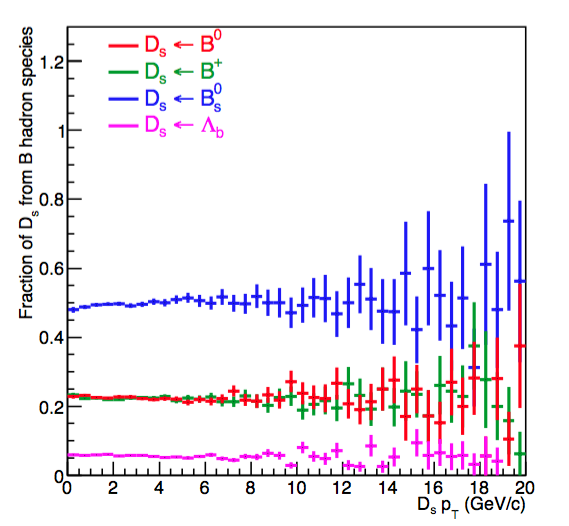
\includegraphics[width=0.5\textwidth]{FigCap4/DsParents.png}
\caption{Fraction of $\Ds$ from $b$-hadron decays.}
\label{fig:DsParents}
\end{center}
\end{figure}
Considering that:
\begin{itemize}
\item FONLL provides a good description of B$^{+}$- and B$^{0}$-meson 
cross-sections at $\s =$ 7 TeV both at mid- and forward rapidity and of 
B feed-down $J/{\rm \psi}$-meson cross-section at forward rapidity at  $\s =$ 7, 8 TeV;
\item FONLL provides a good description also for the 
B$^0_{\rm s}$-meson cross-section at forward rapidity where data are available in a wider $p_{T}$ range 
than at mid-rapidity, allowing for a safer comparison; FONLL also describes 
$\Lambda_{\rm b}$-baryon cross-section, provided 
a rescaling of a factor 2, that may account for 
the large uncertainty of the branching ratio of the channel used in the LHCb analysis;
\end{itemize}
the calculation of $f_{\rm prompt}$ with the method in Eq.~\ref{eq:fpr} is then fully justified.
In fact, as Fig.~\ref{fig:DsParents} shows, around half of B feed-down 
$\Ds$ originates from B$^0$- and B$^+$-meson decays 
and half from B$^0_{\rm s}$-meson decays.
The method in Eq.~\ref{eq:fc}, instead, would suffer from the 
underestimation of charm production at the LHC energies. 
It is reasonable to conclude that, on the basis of the current 
measurements, Eq.~\ref{eq:fc} would artificially introduce a bias if 
used to subtract the beauty feed-down component, thus artificially enhancing 
the systematics uncertainty.


\subsection{Generated $\pt$ shape}

The influence of the shape of the generated $\Ds$ $\pt$ spectrum used in 
Monte Carlo simulations on the efficiency corrections was also evaluated. 
To estimate this contribution, the reconstruction and selection 
efficiency computed with PYTHIA with Perugia-0 tune
were compared to the ones obtained with FONLL calculations. 
This resulted in a systematic effect on the $\Ds$ selection efficiency of $\sim$ 3\% 
in the two lowest $\pt$ intervals and of $\sim$ 2\% at higher transverse momenta.\\

\begin{table}[!tb]
\centering
\begin{tabular}{l|ccccc}
 \hline 
 & \multicolumn{4}{c}{$\pt$ interval ($\GeV/c$)}\\
 & 2--4 & 4--6 & 6--8 & 8--12\\
\hline
Raw yield extraction & 5\%& 5\%& 5\%& 5\%\\
Topol. sel. efficiency & 7\%& 7\%& 7\%& 7\%\\
Tracking efficiency & 5\%& 5.5\% & 6\% & 6\%\\
PID efficiency & 7\%& 7\%& 7\%& 7\%\\
MC $\pt$ shape   &3\%&3\%&2\%&2\%\\
Feed-down from B & $^{+4.1\%}_{-4.6\%}$& $^{+3.7\%}_{-4.7\%}$& $^{+3.8\%}_{-4.8\%}$& $^{+4.0\%}_{-4.8\%}$\\
Luminosity  & \multicolumn{4}{c}{3.5\%} \\
BR  & \multicolumn{4}{c}{3.5\%} \\
\hline 
\end{tabular}
\caption{Relative systematic uncertainties on the $\pt$-differential production
cross section of prompt $\Ds$ mesons.}
\label{tab:SystDs}
\end{table}

\begin{figure}[!b]
\begin{center}
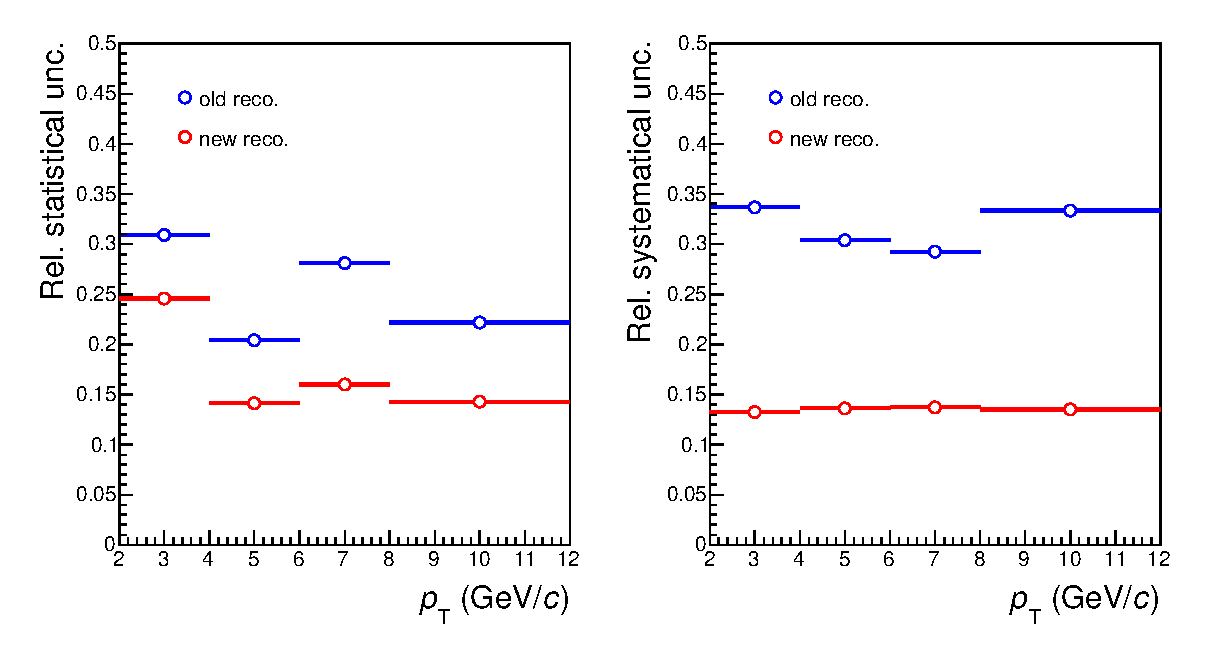
\includegraphics[width=.99\textwidth]{FigCap4/uncertainties_pass2_pass4.eps}
\caption{Comparison of statistical and global systematic uncertainty on $\Dsplus$-meson
cross section in the old reconstruction-based publication and the new analysis~\cite{Acharya:2017jgo}.}
\label{fig:UncNewVsOld}
\end{center}
\end{figure}


The values of the systematic uncertainties above discussed are summarised
in Table~\ref{tab:SystDs}. The uncertainty on the $\Dsplus$-meson production 
cross-section normalisation has a further contribution from the 3.5\%
uncertainty on the minimum-bias trigger cross section~\cite{Abelev:2012sea} 
and a contribution from the uncertainties on the branching ratio (2.27 $\pm$ 0.08 \%)
of the considered decay channel. The systematic uncertainty 
on minimum-bias cross section originates from the uncertainty 
in the determination of the cross section of collisions 
which give signals in both sides of the V0 scintillator detector and 
that was measured by means of van der Meer scan technique~\cite{vanderMeer:296752}.
In Fig.~\ref{fig:UncNewVsOld} the values of statistical and global
systematic uncertainties are shown as a function of $\pt$ and compared to values from 
the analysis of previous reconstruction of this sample.  



\section{Results}
The $\pt$-differential cross sections for prompt $\Ds$ 
production in $|y|<0.5$ are shown in black data points in 
Fig.~\ref{fig:CrossSecDsvsGMVFNS}~\cite{Acharya:2017jgo}.
The error bars represent the statistical uncertainties, while the systematic 
uncertainties are shown as boxes around the data points. 
The symbols are positioned horizontally at the centre of each $\pt$ interval,
with the horizontal bars representing the width of the $\pt$ interval. 
\begin{figure}[!b]
\begin{center}
%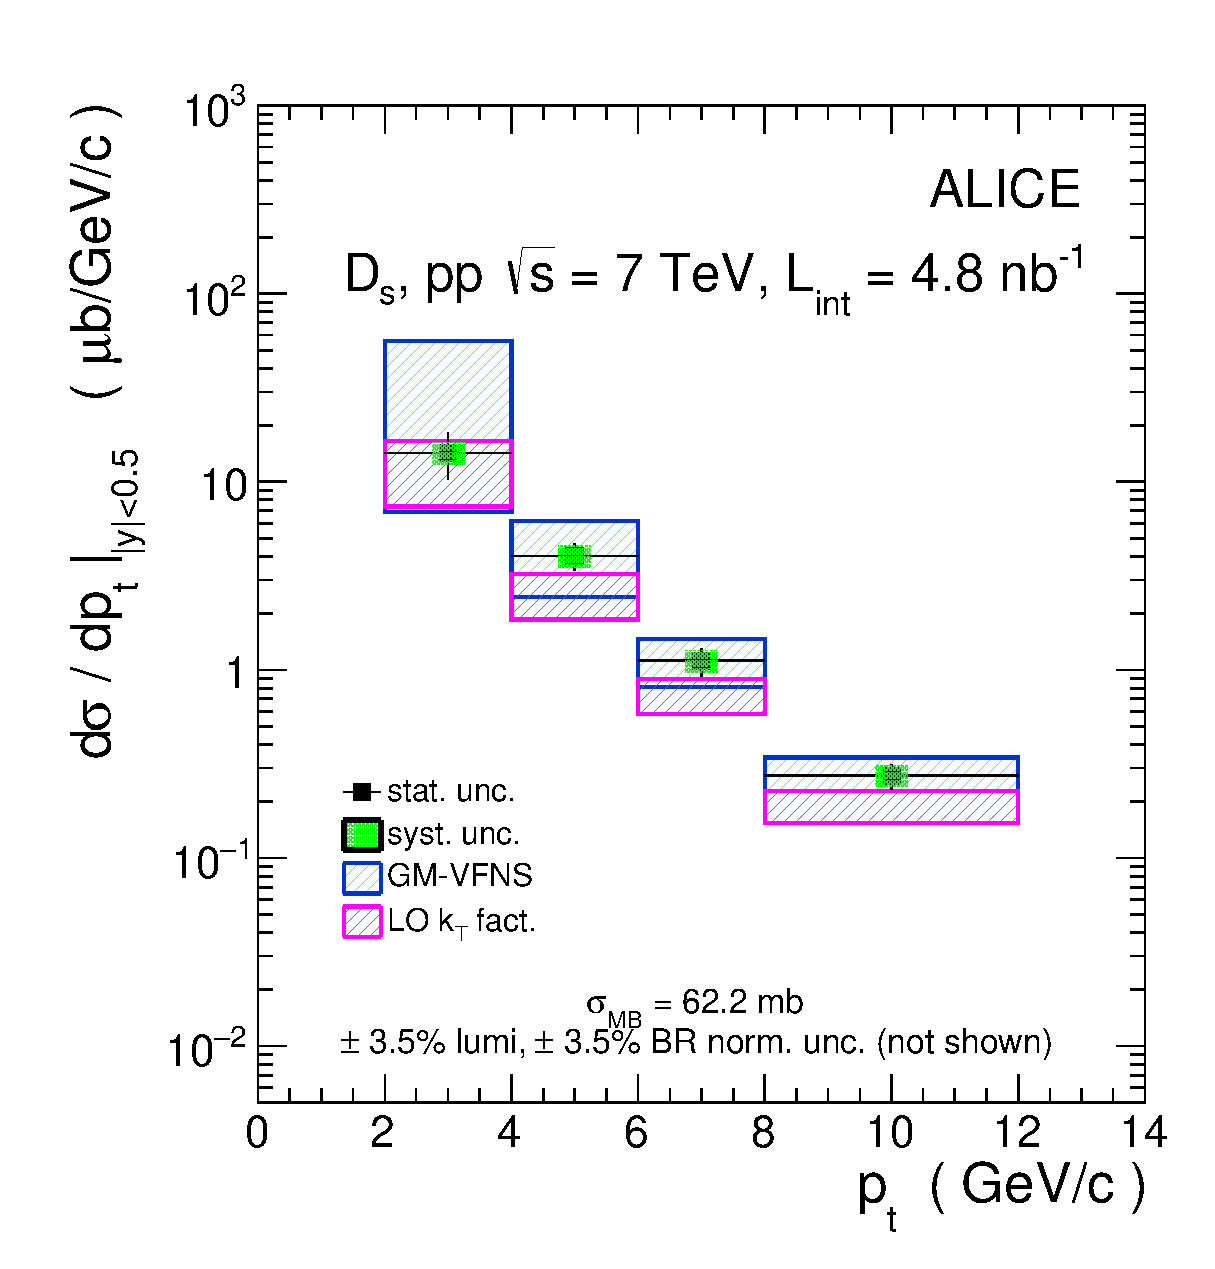
\includegraphics[width=.48\textwidth]{FigCap4/DsCrossModel.eps}
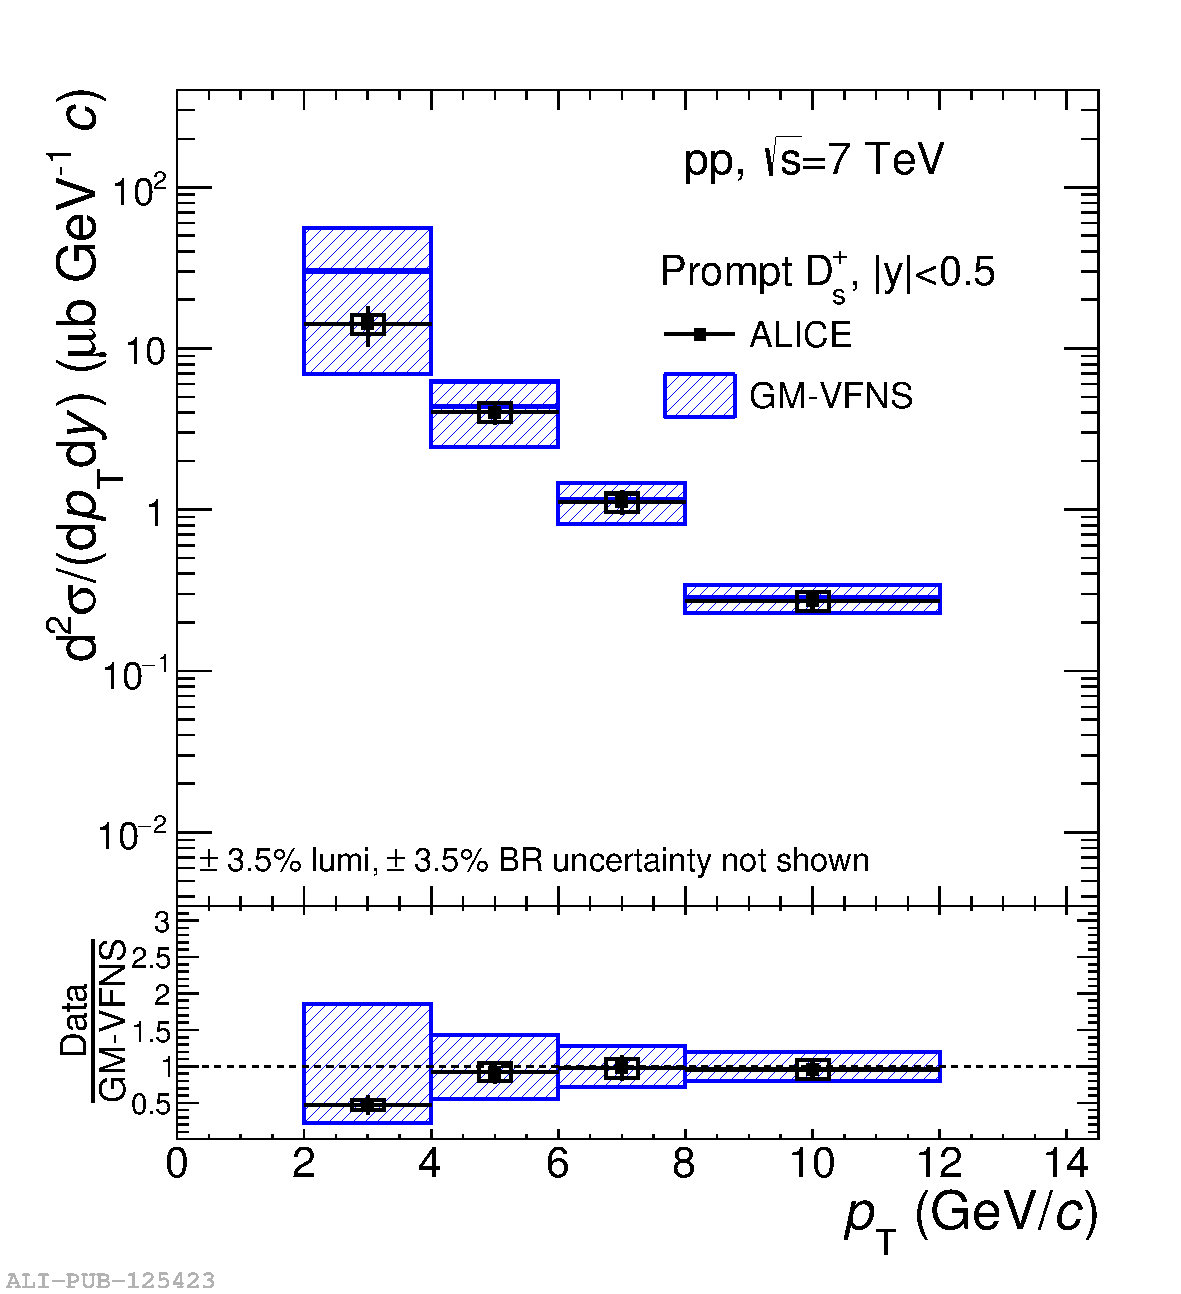
\includegraphics[width=.48\textwidth]{FigCap4/DsppCrossSecVsGMVFNSAndRatio.pdf}
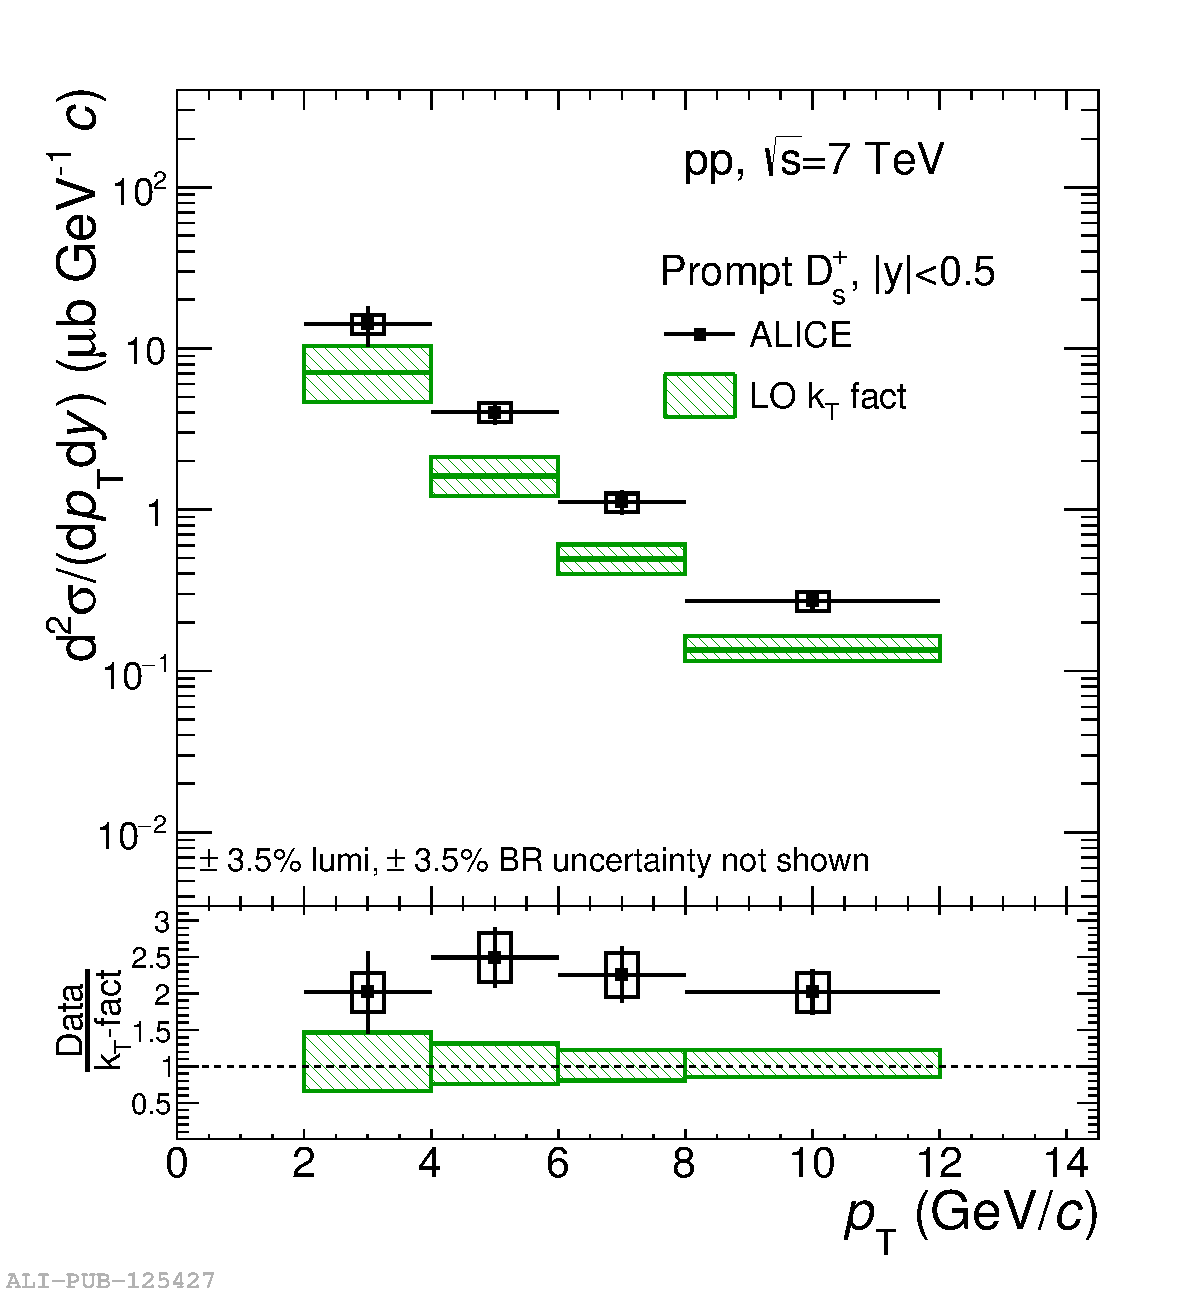
\includegraphics[width=.48\textwidth]{FigCap4/DsppCrossSecVsKtFactAndRatio.pdf}
\caption{$\pt$-differential production cross section of prompt $\Dsplus$ mesons 
with $|y|<0.5$ in the interval \mbox{$2<\pt<12~\gev/c$}, in pp collisions at 
$\s  =$ 7 TeV~\cite{Acharya:2017jgo}. 
The cross section is compared to two pQCD calculations: 
GM-VFNS~\cite{Kniehl:2012ti} (left panel) and a leading order (LO) calculation 
based on $k_{\rm T}$-factorisation~\cite{Maciula:2013wg} (right panel).
}
\label{fig:CrossSecDsvsGMVFNS}
\end{center}
\end{figure}

The results are consistent within uncertainties with 
those reported in the previous publication on charmed-meson 
cross sections in pp collisions at $\s=$ 7 TeV~\cite{ALICE:2011aa,Abelev:2012tca},
but the total uncertainties (sum in quadrature of statistical and systematic
errors) are reduced by a factor 1.5-2, depending on the the $\pt$ interval.
The measured $\pt$-differential cross section is also compared with results from 
perturbative QCD calculations GM-VFNS~\cite{Kniehl:2004fy,Kniehl:2005mk,Kniehl:2012ti}
and $k_{\rm T}$-factorisation~\cite{Maciula:2013wg}.
The results of these calculations, performed in the same $\pt$ intervals of the 
measurement, are shown as filled boxes spanning the theoretical uncertainties
and a solid line representing the values obtained with the central values of 
the pQCD parameters.
The theoretical uncertainties are estimated in the two frameworks
by varying the renormalisation and factorisation scales. 
In $k_{\rm T}$-factorisation calculations also the effect of the 
charm-quark mass uncertainty is considered.
In the GM-VFNS calculations, the CTEQ6.6 PDFs~\cite{Pumplin:2002vw}
were used. The LO $k_{\rm T}$-factorisation calculations were performed
with an updated set of unintegrated gluon-distribution functions computed 
from the recent MMHT2014-LO PDFs~\cite{Harland-Lang:2014zoa}.
The central value of the LO $k_{\rm T}$-factorisation predictions lies systematically 
below the data.
The GM-VFNS calculations describe the data within 
uncertainties for $\pt>4~\gev/c$, while in the interval
$2<\pt<4~\gev/c$ the predictions overestimate the measured production
cross sections.\\


\begin{figure}[!htb]
\begin{center}
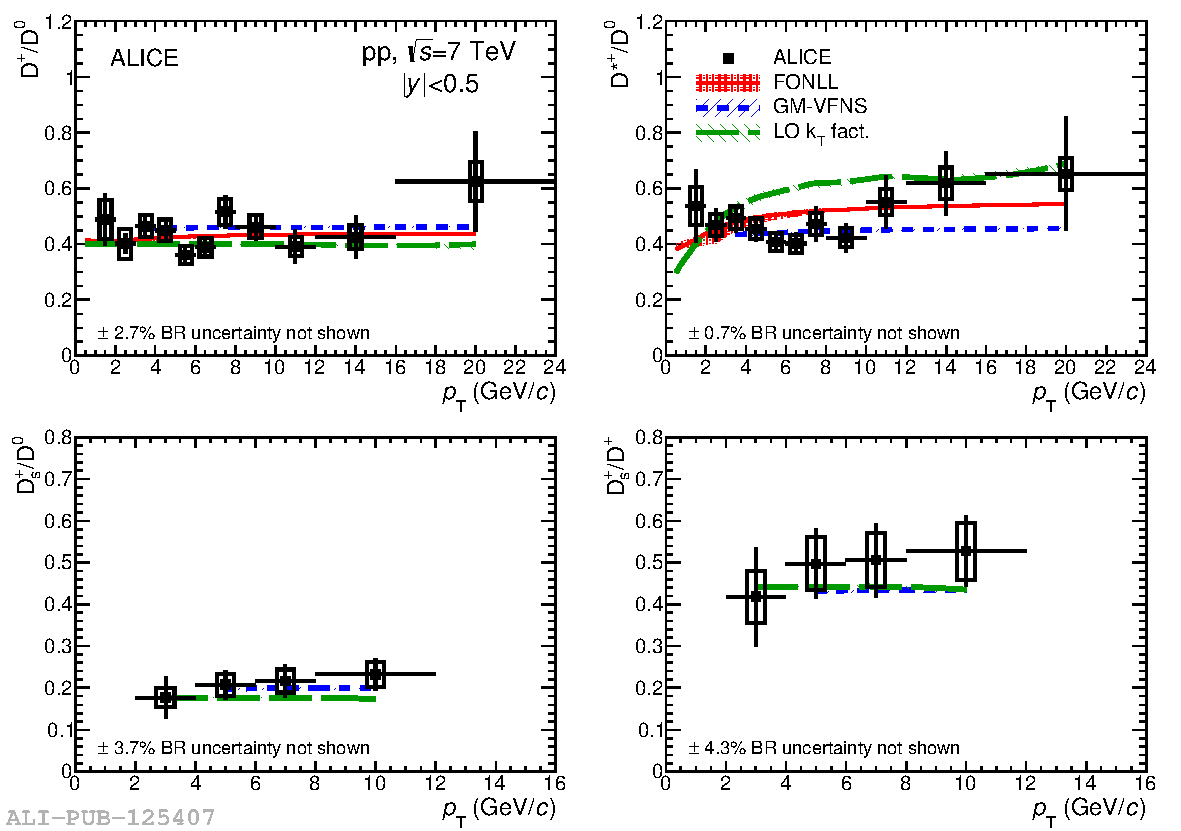
\includegraphics[width=1\textwidth]{FigCap4/DmesonRatiosVsModels.pdf}
\caption{Ratios of D-meson production cross sections as a function of $\pt$~\cite{Acharya:2017jgo}.
Predictions from FONLL, GM-VFNS and LO $\kt$-factorisation calculations
are also shown. For the pQCD calculations the line shows the ratio of
the central values of the theoretical cross sections, while the shaded area is 
defined by the ratios computed from the upper and lower limits of the 
theoretical uncertainty band.}
\label{fig:DratiosVsPt}
\end{center}
\end{figure}



The ratios of the $\pt$-differential cross sections of $\Dzero$, $\Dplus$, 
$\Dstar$ and $\Ds$ mesons are reported in Fig.~\ref{fig:DratiosVsPt}~\cite{Acharya:2017jgo}.
In the evaluation of the systematic uncertainties on these ratios, 
the sources of correlated and uncorrelated systematic effects were treated 
separately. In particular, the contributions of the yield extraction and cut efficiency 
were considered as uncorrelated, while those of the feed-down from 
beauty-hadron decays and the tracking efficiency were treated as fully 
correlated among the different D-meson species.
The measured D-meson ratios do not show a significant $\pt$ dependence within 
the experimental uncertainties, thus suggesting a small difference 
between the fragmentation functions of charm quarks to pseudoscalar 
($\Dzero$, $\Dplus$ and $\Ds$) and vector ($\Dstar$) mesons and to strange and 
non-strange mesons.
The data are compared to the ratios of the D-meson cross sections from FONLL 
(only for $\Dzero$, $\Dplus$ and $\Dstar$ mesons), GM-VFNS and LO 
$\kt$-factorisation pQCD calculations.
The ratios of the theoretical predictions were computed assuming their 
uncertainties to be fully correlated among the D-meson species, which 
results in an almost complete cancellation of the uncertainties in the ratio. 
Note that in all these pQCD calculations, the relative abundances of the 
different D-meson species are not predicted by the theory, but 
the fragmentation fractions, $f({\rm c\rightarrow D})$, are taken from 
the experimental measurements~\cite{Kneesch:2007ey,Cacciari:2012ny,Cacciari:2003zu,Maciula:2013wg,Barate:1999bg,Gladilin:2014tba}.
In the FONLL and GM-VFNS frameworks, the $\pt$ dependence 
of the ratios of the D-meson production cross sections arises from the 
different fragmentation functions used to model the transfer of energy from 
the charm quark to a specific D-meson 
species~\cite{Cacciari:2003zu,Kneesch:2007ey,Kniehl:2006mw}, 
and from the different contribution from decays of higher excited states.
The parton fragmentation models used in the calculations provide
an adequate description of the measured data.
In the LO $\kt$-factorisation calculations, the same fragmentation function 
(Peterson~\cite{Peterson:1982ak}) is used for $\Dzero$, $\Dplus$ and $\Ds$ 
mesons, resulting in the same shape of the $\pt$ distributions of these three 
meson species, while 
the fragmentation functions for vector mesons from Ref.~\cite{Braaten:1994bz} 
are used for $\Dstar$ mesons~\cite{Maciula:2013wg}.

